\documentclass[oneside, 12pt]{book}     

%% Language and font encodings
\usepackage[english]{babel}
\usepackage[utf8x]{inputenc}
\usepackage[T1]{fontenc}
\usepackage{amsfonts}
\usepackage[margin=30mm]{geometry}

%% Sets page size and margins
%\usepackage[a4paper,top=3cm,bottom=2cm,left=3cm,right=3cm,marginparwidth=1.75cm]{geometry}

%% Useful packages
\usepackage[colorlinks=true, allcolors=black]{hyperref}
\usepackage{amsmath}
\usepackage{xcolor}
\usepackage{amssymb}
\usepackage{amsthm}
\usepackage{stmaryrd}
\usepackage{graphicx}
\usepackage{enumitem}
\usepackage{multicol}
\usepackage{tikz, pgfplots}
\usepgfplotslibrary{fillbetween}
\usepackage{hyperref}
\usetikzlibrary{positioning}

%Theorem
\theoremstyle{plain}
\newtheorem{theorem}{Theorem}[section]
\newtheorem{proposition}[theorem]{Proposition}
\newtheorem{lemma}[theorem]{Lemma}
\newtheorem*{corollary}{Corollary}
\theoremstyle{definition}
\newtheorem*{definition}{Definition}
\newtheorem{exercise}[theorem]{Exercise}
\newtheorem*{exercise*}{Exercise}

%Usual Sets
\newcommand{\C}{\mathbb{C}}
\newcommand{\R}{\mathbb{R}}
\newcommand{\Q}{\mathbb{Q}}
\newcommand{\Z}{\mathbb{Z}}
\newcommand{\N}{\mathbb{N}}
\newcommand{\F}{\mathbb{F}}
\newcommand{\E}{\mathbb{E}}
\newcommand{\K}{\mathbb{K}}
\newcommand{\Zn}[1]{\mathbb{Z}/ #1 \mathbb{Z}}

%Special Sets
\newcommand{\Iint}[2]{\llbracket #1 , #2 \rrbracket}

%Math Operators
\let\Re\relax
\let\Im\relax
\DeclareMathOperator{\Im}{Im}
\DeclareMathOperator{\Re}{Re}
\DeclareMathOperator{\Null}{null}
\DeclareMathOperator{\range}{range}
\DeclareMathOperator{\card}{card}
\DeclareMathOperator{\Aut}{Aut}
\DeclareMathOperator{\Hom}{Hom}
\DeclareMathOperator{\Gal}{Gal}
\DeclareMathOperator{\Char}{char}

%Other Symbols
\newcommand{\td}{\textcolor{red}{\textbf{TODO}}}
\newcommand{\isomorphic}{\cong}

% Equations
\numberwithin{equation}{section}

%Set QED symbol to blacksquare
\renewcommand\qedsymbol{$\blacksquare$}

\title{\Huge Motivating L-functions}
\author{Samy Lahlou}
\date{}

%\includeonly{EulerMarvelousSeries/SummationFormula/summationFormula,
%EulerMarvelousSeries/BaselProblem/baselProblem.tex,
%EulerMarvelousSeries/PrimeNumbers/PrimeNumbers.tex,
%EulerMarvelousSeries/BernoulliNumbers/BernoulliNumbers.tex}
%\includeonly{EulerMarvelousSeries/CuriousRatio/CuriousRatio}

\pgfplotsset{compat=1.18}

\begin{document}

\maketitle 

\frontmatter

%PREFACE
\chapter*{Preface}
\addcontentsline{toc}{chapter}{Preface}

This document is my report for my Summer 2025 NSERC under the supervision of Professor Henri Darmon at McGill University. My goal with this document is to motivate the concept of L-functions and highlight some of its applications to show the deep connections between L-functions and Number Theory. To motivate the theory, I will first deeply focus on the historical motivations, and then present some more modern results such as the connections with elliptic curves and modular forms, or more generally, the Langlands program.

The first chapter will focus on Leonhard Euler. I believe that the historical motiva-tions for the theory of L-functions can be traced back to the work of Euler more than any other mathematician. I will first present his summation formula which he used extensively. After that, I will present his solution(s) to the Basel Problem but also the link he made with some particular series and the prime numbers. I will then finish the chapter with important results that involve the Bernoulli numbers and what will become the functional equations of some L-functions. I will add more informations about the other chapters once I will finish writing them.

Beside the structure of this report, there are three things I find very important to keep in mind while reading this document:
\begin{itemize}
    \item My goal is to preserve the authenticity of the results that will be presented. Hence, I will use the original notation and the original terms as much as possible. For example, in the first chapter, I will avoid using the symbol $\sum a_n$ for sums and use $a_1 + a_2 + a_3 + \dots$ instead. Similarly, I will not talk about \textit{real numbers} or \textit{sets} as this notion didn't exist until the very end of the 19th century. Moreover, I will also state and prove the theorems that are presented as they were stated and proved. Thus, the proofs that I will present will always be the original proofs with very little modifications.
    \item The Bernoulli numbers will be mentionned for the first time in \autoref{sec: bernoulli numbers} and will probably be used a lot in the rest of the document. It is important to keep in mind that in modern number theory books, the Bernoulli number $B_1$ is sometimes defined as $+1/2$ and sometimes defined as $-1/2$. In this document, I will assume that $B_1 = + 1/2$ for very good reasons that I will expose in \autoref{sec: bernoulli numbers}.
    \item I made the decision of adding exercises at the end of each section because I strongly believe that it really helps understanding the content of the section. There are two types of exercises: the first type will be exercises outlining some results from papers that are presented in the section but that I didn't get time to present or prove, the second type will be exercises that outline a rigorous or alternative proof of a result that appears in the section. Some important results have non-rigorous or false proofs, hence, the second type of exercise will help using these results in the latter chapters without having doubts about their validity.
\end{itemize}

The prerequisites for this document would be some familiarity with Real and Complex Analysis, Abstract Algebra (especially Group Theory) and Elementary Number Theory (properties of prime numbers, congruences, ...). Besides these prerequisites, the document contains appendices that should make it self-contained.

It is more than possible that I made some mistakes. Feel free to correct me or ask me anything about the content of this document at the following email address : \href{mailto:samy.lahloukamal@mail.mcgill.ca}{samy.lahloukamal@mail.mcgill.ca}.

\tableofcontents

\newpage

%CHAPTERS
\mainmatter

%CHAPTER 1: EULER
\chapter{Euler's Marvelous Series}

\section{Euler's Summation Formula}

The Calculus developed by Sir Isaac Newton (1643 - 1727) and Gottfried Wilhelm Leibniz (1646 - 1716) at the end of the 17th century made the subject of infinite series very popular and useful in mathematics. Before this era, the concept of infinite sums was already encountered in different places in the world. For example, in a treatise written by Archimedes of Syracuse (287 BC - 212 BC) in the 3rd century BC called \textit{Quadrature of the Parabola} \cite{archimedes1897}, there is a visual proof that
$$\frac{1}{4} + \frac{1}{16} + \frac{1}{64} + \frac{1}{256} + \dots = \frac{1}{3}$$
using embedded squares. Next, the decimal representation of numbers, which was introduced in Europe during the 13th century, is simply an application of infinite sums in disguise. For example, the fact that $1/3$ has the decimal expansion $0.333333\dots$ can be reinterpreted as saying that
$$\frac{1}{3} = \frac{3}{10} + \frac{3}{10^2} + \frac{3}{10^3} + \frac{3}{10^4} + \frac{3}{10^5} + \dots$$
In the 14th century, the French mathematician Nicole Oresme (1320 - 1382) showed that the infinite sum
$$1 + \frac{1}{2} + \frac{1}{3} + \frac{1}{4} + \frac{1}{5} + \dots$$
has an infinite value in the sense that it exceeds any finite quantity. As Archimedes, using a geometric argument, he was able to find the following results:
\begin{align*}
    1 + \frac{1}{2} + \frac{1}{4} + \frac{1}{8} + \frac{1}{16} + \dots &= 2 \\
    \frac{1}{2} + \frac{2}{4} + \frac{3}{8} + \frac{4}{16} + \frac{5}{32} + \dots &= 2
\end{align*}
More informations about the work of Nicole Oresme can be found in the article \textit{Mathematical Concepts and Proofs from Nicole Oresme} \cite{NicoleOresme}. 

Later, between the 14th and 15th century, members of the Kerala school of astronomy and mathematics, in India, found representations of the sine and the cosine of an angle as an infinite sum. They also found an infinite sum representation of the arctangent of a given quantity. In modern notation, these results can be written as follows:
\begin{equation}
    \sin(\theta) = \theta - \frac{\theta^3}{3!} + \frac{\theta^5}{5!} - \frac{\theta^7}{7!} + \dots
\end{equation}
\begin{equation}
    \cos(\theta) = 1 - \frac{\theta^2}{2!} + \frac{\theta^4}{4!} - \frac{\theta^6}{6!} + \dots
\end{equation}
\begin{equation} \label{Madhava arctan}
    \arctan(x) = x - \frac{x^3}{3} + \frac{x^5}{5} - \frac{x^7}{7} + \dots
\end{equation}
These three equations are sometimes called Madhava Series in reference to the Indian mathematician Madhava of Sangamagrama (1340 - 1425), a member of the Kerala school to which these results are attributed. Moreover, by plugging-in $x=1$ in equation (\ref{Madhava arctan}), the following equation is obtained:
\begin{equation} \label{Leibniz / Madhava Series}
    \frac{\pi}{4} = 1 - \frac{1}{3} + \frac{1}{5} - \frac{1}{7} + \frac{1}{9} - \frac{1}{11} + \dots
\end{equation}
This equation was later rediscovered independently by Leibniz which is the reason why people usually call equation (\ref{Leibniz / Madhava Series}) the Leibniz Series. More informations about this result can be found in the article \textit{The Discovery of the Series Formula for $\pi$ by Leibniz, Gregory and Nilakantha} \cite{LeibnizMadhavaSeries}. Compared to the previously discussed results, this one has a particular importance since it involves the constant $\pi$ even though the infinite sum on the right hand side doesn't seem more complicated than the ones discussed above. This result is a first hint that some seemingly simple infinite sums can have unexpected behaviors.

Finally, in 1650, the Italian mathematician Pietro Mengoli (1626 - 1686) publishes his book \textit{Novæ quadraturæ arithmeticæ, seu de additione fractionum} \cite{mengoli1650nouæ} in which he proves various results about infinite sums. For example, he proves that the Harmonic Series is infinite, and also finds the values of
$$\frac{1}{1\cdot(1 + r)} + \frac{1}{2\cdot(2 + r)} + \frac{1}{3\cdot(3 + r)} + \frac{1}{4\cdot(4 + r)} + \dots$$
where $r$ is any integer between 1 and 10. However, he was unable to find the value to which the series
$$\frac{1}{1^2} + \frac{1}{2^2} + \frac{1}{3^2} + \frac{1}{4^2} + \dots$$
converges to (which is the case $r=0$ of the previous sums). Thus, we see through these examples that before the works of Newton and Leibniz, infinite sums already made their appearance in various contexts in time.

Even though some specific examples of infinite sums were already studied in the previous centuries, they really became central in  mathematics when the tools of calculus became available. For example, with his method of fluxions, Newton rediscovered the Madhava Series for the sine and cosine functions and was able to solve differential equations. The tools of calculus gave the perfect framework for what is begining to be called series or infinite series.

Later in that period, in 1689, the Swiss mathematician Jakob Bernoulli (1655 - 1705) wrote his \textit{Tractatus de seriebus infinitis}, a treatise on infinite series in which he discusses the limiting values of various series such as geometric series, telescoping series, the harmonic series and other types of series. For example, he derives the following formula for geometric series:
\begin{equation}
    a + ar + ar^2 + ar^3 + \dots = \frac{a}{1-r}, \qquad \quad -1 < r < 1.
\end{equation}
He also studied some more specific examples such as
\begin{equation}\label{telescoping series}
    \begin{split}
        & 1 + \frac{1}{3} + \frac{1}{6} + \frac{1}{10} + \frac{1}{15} + \frac{1}{21} + \frac{1}{28} + \dots \\
        & = \frac{2}{1(1+1)} + \frac{2}{2(2+1)} + \frac{2}{3(3+1)} + \frac{2}{4(4+1)} + \dots = 2
    \end{split}
\end{equation}
using the fact that it is a telescoping series. As his predecessors, he gave a new proof of the divergence of the Harmonic Series. Finally, when considering the series of the reciprocals of the squares 
$$\frac{1}{1^2} + \frac{1}{2^2} + \frac{1}{3^2} + \frac{1}{4^2} + \dots,$$
he was able to show that it must have a finite limiting value, i.e., that the series converges, by using the inequality 
$$\frac{1}{n^2} \leq \frac{2}{n(n+1)}$$
and combining it with equation (\ref{telescoping series}) to obtain
$$1 + \frac{1}{4} + \frac{1}{9} + \frac{1}{16} + \dots \leq 1 + \frac{1}{3} + \frac{1}{6} + \frac{1}{10} + \dots = 2 < \infty.$$
However, he was unable to find the precise value to which the series converges to and wrote in his \textit{Tractatus} that "great will be our gratitude" if anyone finds and communicates this limiting value. This became known as the Basel Problem, since the mathematician wrote from Basel in Switzerland, and it remained unsolved for decades.

Let's notice that this series converges very slowly since the individual terms don't approach zero fast enough. This is a problem because a good strategy to find the value of a series is to find the sum of the first 20 terms (for example) and guess the limit of the series from this approximation. However, with the series of the reciprocals of the squares, taking the sum of the first 200 terms gives an approximation which is only correct for one decimal. Hence, it makes the problem even harder to solve.

The first mathematician to make some progress on the Basel Problem is a young Swiss mathematician which had Johann Bernoulli (1667 - 1748), Jakob Bernoulli's younger brother, as his mathematics professor. This young mathematician quickly learned the mathematics of his time and would soon become the most prolific mathematician of all time. This mathematician is obviously the great Leonhard Euler (1707 - 1783). 

Euler's first contribution to the Basel Problem can be found in his article \textit{De summatione innumerabilium progressionum} \cite{eulerE20} which he wrote in 1731 and published in 1738. In this article, using many integral tricks and algebraic manipulations, Euler is able to obtain the formula
$$\frac{1}{1^2} + \frac{1}{2^2} + \frac{1}{3^2} + \frac{1}{4^2} + \dots = \left(\frac{1}{2^0\cdot 1^2} + \frac{1}{2^1\cdot 2^2} + \frac{1}{2^2\cdot 3^2} + \frac{1}{2^3\cdot 4^2} + \dots \right) + (\ln 2)^2$$
which relates the series of the reciprocals of the squares to a series which converges much faster to which is added a constant term which can be computed very precisely. With only 20 terms of the right hand side series, Euler is able to obtain the following approximation:
$$1 + \frac{1}{4} + \frac{1}{9} + \frac{1}{16} + \frac{1}{25} + \dots = 1.644934$$
He notices himself that such an approximation can only be obtained by adding more than a thousand terms of the series on the left hand side. Using computers, it turns out that such an approximation would require to sum more than 15 millions terms of the original series, which makes this result already very remarkable. Again, this shows how slowly the original series converges.

Three years later, in the article \textit{Methodus universalis serierum convergentium summas quam proxime inveniendi} \cite{eulerE46} written in June 1735 and published in 1741, Euler found another way of approximating the sum of the reciprocals of the squares. His method was a general method for approximating series using their integral representation. At the end of the paper, he applied his method to the series of the reciprocals of the square. His method was very geometric. He considered the following figure

\begin{figure}[h]
    \centering
      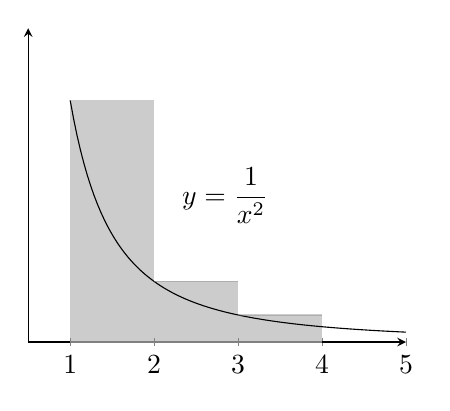
\begin{tikzpicture}[scale=0.7]
        \begin{axis}[
            axis lines = left,
            xmin=0.5,
            ymin=0,
            ymax=1.3,
            ymajorticks=false
        ]
    
        \addplot [domain=1:5, samples=100, color=black,] {(1/x^2) + 0.001} node[above=1cm, pos=0.5] {$\displaystyle y = \frac{1}{x^2}$};
    
        \addplot [domain=1:2,samples=2, color=gray, opacity=0.4, name path=f1,]{1};
        \addplot [domain=1:2,samples=2, color=gray, name path=g1,]{0};
        \addplot[gray, opacity=0.4] fill between[of=f1 and g1, soft clip={domain=1:2}];
    
        \addplot [domain=2:3,samples=2, color=gray, opacity=0.4, name path=f2,]{0.251};
        \addplot [domain=2:3,samples=2, color=gray, name path=g2,]{0};
        \addplot[gray, opacity=0.4] fill between[of=f2 and g2, soft clip={domain=2:3}];
    
        \addplot [domain=3:4,samples=2, color=gray, opacity=0.4, name path=f3,]{0.1121};
        \addplot [domain=3:4,samples=2, color=gray, name path=g3,]{0};
        \addplot[gray, opacity=0.4] fill between[of=f3 and g3, soft clip={domain=3:4}];
        
        \end{axis}
    \end{tikzpicture}
    \caption{Visual interpretation of}
    \text{$1 + \frac{1}{2^2} + \frac{1}{3^2} + \frac{1}{4^2} + \dots$}
    \label{fig:visual sum vs integral}
\end{figure}

in which the shaded area represents the value of the sum of the reciprocals of the squares. We can see that this sum is greater than the area under the curve $y = \frac{1}{x^2}$ between $x=1$ and $x = \infty$. But Euler's goal was to approximate the shaded area above the curve. Using some calculus and geometry, he was able to derive the following approximation of the total shaded area:
$$1 + \frac{1}{4} + \frac{1}{9} + \frac{1}{16} + \frac{1}{25} + \dots = 1.644920$$
which is only true for the first four decimals. It seems like this method is worst than the previous one since it only gives an approximation true for the first four decimals. However, Euler was on track to develop a new very powerful method.

As for the previous method, Euler's goal was to approximate the difference between a series and the integral of the general term of the series. In his paper \textit{Methodus generalis summandi progressiones} \cite{eulerE25}, written in 1732 and published in 1738, Euler mentions without proof such a formula that links a series to its corresponding integral. He then wrote another article called \textit{Inventio summae cuiusque seriei ex dato termino generali} \cite{eulerE47}, written in October 1735 and published in 1741, to go over the proof of his formula and apply it to approximate some series. Let's dive into this last paper to understand his formula. 

The paper starts with an important preliminary result. Take a function $y$ of $x$ which can be expanded as follows:
$$y(x) = a_0 + a_1x + a_2x^2 + a_3x^3 + a_4x^4 + \dots,$$
then for any $\alpha$, by the Binomial Theorem:
\begin{align*}
    y(x+\alpha) &= \ a_0 \\
    &+ \left(a_1 x \ \, \, \! + a_1 \alpha\right) \\
    &+ \left(a_2 x^2 + 2a_2 x \alpha \ \ \!+ a_2 \alpha^2\right) \\
    &+ \left(a_3 x^3 + 3a_3 x^2 \alpha + 3 a_3 x\alpha^2 \, \, \,  + a_3 \alpha^3\right) \\
    &+ \left(a_4 x^4 + 4a_4 x^3 \alpha + 6 a_4 x^2 \alpha^2 + 4 a_4 x \alpha^3 + a_4 \alpha^4 \right) \\
    &+ \dots
\end{align*}
Now, if we sum the right hand sum column by column, we obtain
\begin{align*}
    y(x+\alpha) &= (a_0 + a_1 x + a_2 x^2 + a_3 x^3 + a_4 x^4 + \dots) \\
    &+ \alpha(a_1 + 2a_2x + 3a_3 x^2 + 4 a_4 x^3 + \dots) \\
    &+ \frac{\alpha^2}{2}(2a_2 + 3\cdot 2 a_3x + 4\cdot 3 a_4 x^2 + \dots)
\end{align*}

considering the following set-up. If $f$ is a function of $x$, then we can define
\begin{equation}
    S(x) = f(1) + f(2) + f(3) + \dots + f(x)
\end{equation}
which is also a function of $x$. The goal now is to find a simpler way of expressing $x$. For example, if $f(x) = x$, then $S(x)$ is simply $x(x+1)/2$. 

\td \\

\noindent {\Large\textbf{Exercises}}

\begin{exercise}
    In this exercise, the sequence $H_n = \sum_{k=1}^{n}\frac{1}{k}$ denotes the sequence of partial sums of the Harmonic Series. In the article \textit{De summatione innumerabilium progressionum} written in 1731, Euler interpolated the sequence $H_n$ using the function
    $$H(x) = \int_{0}^{1}\frac{1-t^x}{1-t}dt.$$
    \begin{enumerate}[label=(\alph*)]
        \item Prove that $H(n) = H_n$ for all $n \geq 1$.
        \item Find the value of $H(1/2)$.
        \item Prove that $H(x + 1) = H(x) + \frac{1}{x+1}$ for all $x > 0$.
        \item Deduce a general formula for $H(n + \frac{1}{2})$. 
    \end{enumerate}
\end{exercise}

\td 

\begin{enumerate}
    \item Faire un exercise qui outline une simplification de la preuve de Euler de la formule avec ln2 au carré et la série qui converge plus rapidement.
    \item Faire un exercise sur les approximations de Euler de la série harmonique issu de son deuxième papier de 1735.
\end{enumerate}

\td 
\section{Solving the Basel Problem} \label{sec: Basel Problem}

We ended last section with Euler's astonishing approximation of the sum of the recipro-cals of the squares. However, an approximation is still an approximation, the Basel Problem is still far from being solved. Or is it ? As it was said at the end of the previous section, from his approximation, Euler was finally able to see the light and understand the true nature of the sum of the reciprocals of the squares. But what could he notice from these 20 mysterious decimals ?

At that time, the values of both the Leibniz Series and the Alternating Harmonic Series were known:
\begin{align}
    1 - \frac{1}{3} + \frac{1}{5} - \frac{1}{7} + \frac{1}{9} - \frac{1}{11} + \dots &= \frac{\pi}{4} \\
    1 - \frac{1}{2} + \frac{1}{3} - \frac{1}{4} + \frac{1}{5} \, - \, \frac{1}{6} \, + \dots &= \ln 2
\end{align}
Thus, by squaring both sides of both equations could imply that the sum of the reciprocals of the squares can be written in terms of $\pi^2$, $(\ln 2)^2$, or both. Moreover, as we saw in the previous section, Euler already managed to write the sum of the reciprocals of the squares in terms of $(\ln 2)^2$ in equation (\ref{zeta 2 and (ln 2)^2}). These results narrow our possible guesses a lot. This is probably what Euler had in mind because after approximating the desired sum up to 20 decimals, he quickly recognized this value to be... $\pi^2/6$ ! But this is not even the most surprising part, there is still an important question that remains unanswered: why would the sum of the reciprocals of the squares converge to $\pi^2/6$ ?

Euler came up and wrote his (first) proof of this result in December 1735 in the paper \textit{De summis serierum reciprocarum} \cite{eulerBaselProblem} published in 1740. The goal of this section is to understand Euler's proof in details. Let's begin.

\subsection*{The Proof}

First, for a fixed $y$ between $-1$ and $1$, he considered the equation $y = \sin(s)$ where $s$ is a variable. Using the series expansion of the sine function, this equation can be rewritten as
\begin{equation} \label{y = s - s^3/3!}
    y = s - \frac{s^3}{1\cdot 2 \cdot 3} + \frac{s^5}{1\cdot 2\cdot 3 \cdot 4 \cdot 5} - \dots
\end{equation}
Now, Euler noticed that if $y$ is supposed to be non-zero, then dividing by both sides by $y$ and putting all the terms on one side of the equation leads to the key equation
\begin{equation} \label{key equation 1735}
    0 = 1 - \frac{s}{y} + \frac{s^3}{1\cdot 2 \cdot 3\cdot y} - \frac{s^5}{1\cdot 2\cdot 3 \cdot 4 \cdot 5 \cdot y} + \dots
\end{equation}
Next, he viewed this equation as an infinite-degree polynomial equation in $s$, and hence treated the right hand side of equation (\ref{key equation 1735}) as a regular polynomial. Recall that given a polynomial $P(s)$ of finite degree $n$ with roots $a_1, ..., a_n$ and such that $P(0) = 1$, then we can write $P(s)$ as 
\begin{equation} \label{factorization finite polynomial}
P(s) = \left(1 - \frac{s}{a_1}\right)\left(1 - \frac{s}{a_2}\right) \dots \left(1 - \frac{s}{a_n}\right).
\end{equation}
This comes from the fact that the expression on the right hand side of equation (\ref{factorization finite polynomial}) is a polynomial of degree $n$ that has the same roots as $P(s)$ and that has the same value at 0. Since both polynomial coincide on $n+1$ points, then they must be strictly equal. Thus, if we denote by $A$, $B$, $C$, $D$, ... the roots of equation (\ref{key equation 1735}), then Euler extended the previous principle to the infinite case to obtain the following important equation:
\begin{equation} \label{equality between series and product}
    1 - \frac{s}{y} + \frac{s^3}{1\cdot 2 \cdot 3\cdot y} - \frac{s^5}{1\cdot \cdot \cdot 5 \cdot y} + \dots = \left(1 - \frac{s}{A}\right)\left(1 - \frac{s}{B}\right)\left(1 - \frac{s}{C}\right) \dots
\end{equation}
Finally, he defined $A$ to be the least positive root of the equation $y = \sin(s)$, and observed that the roots of the equation are precisely the sequence $A$, $\pi - A$, $-\pi - A$, $2\pi + A$, $-2\pi + A$, $3\pi - A$, $-3\pi - A$, ... which implies that the previous equation can be rewritten as 
\begin{multline}
    1 - \frac{s}{y} + \frac{s^3}{1\cdot 2 \cdot 3\cdot y} - \frac{s^5}{1\cdot \cdot \cdot 5 \cdot y} + \dots \\
    = \left(1 - \frac{s}{A}\right)\left(1 - \frac{s}{\pi - A}\right)\left(1 - \frac{s}{-\pi - A}\right)\left(1 - \frac{s}{2\pi + A}\right)\left(1 - \frac{s}{-2\pi + A}\right) \dots
\end{multline}
From this equation, Euler observed that by expanding the infinite product on the right hand side, the coefficient in front of $s$ on the left hand side is equal to the sum of the terms of the sequence $-\frac{1}{A}$, $-\frac{1}{\pi - A}$, ..., the coefficient in front of $s^2$ on the left hand side is equal to the sum of the factors of two terms in the same sequence, and more generally, that the coefficient in front of $s^n$ on the left hand side is equal to the sum of the factors of $n$ elements in the sequence $-\frac{1}{A}$, $-\frac{1}{\pi - A}$, ... It follows that
\begin{equation} \label{formula for y}
    \frac{1}{y} = \frac{1}{A} + \frac{1}{\pi - A} + \frac{1}{-\pi - A} + \frac{1}{2\pi + A} + \frac{1}{-2\pi + A} + \dots
\end{equation}
With this equation in hand, Euler considered the case where $y = 1$, from which he concluded that the least positive root of the equation $\sin(s) = 1$ is $A = \pi / 2$. Thus, by plugging-in $y=1$ and $A = \pi / 2$ in equation (\ref{formula for y}), he obtained
\begin{equation} \label{pre Leibniz Series}
    1 = \frac{2}{\pi} + \frac{2}{\pi} - \frac{2}{3\pi} - \frac{2}{3\pi} + \frac{2}{5\pi} + \frac{2}{5\pi} + \dots
\end{equation}
which is equivalent to
\begin{equation} \label{Leibniz Series}
    \frac{\pi}{4} = 1 - \frac{1}{3} + \frac{1}{5} - \frac{1}{7} + \frac{1}{9} - \dots
\end{equation}
Euler knew that his method was not perfectly rigorous but this first result was a way for him to confirm that his method works since it recovers some known formulas. Next, Euler recalled one last crucial fact about series. Given a series $\alpha = a + b + c + d + \dots$, if we let $\beta = ab + ac + ad + \dots + bc + bd + \dots + cd + \dots$ be the series of factors from two terms of the sequence $a,b,c,d, ...$, then 
\begin{equation} \label{series of squares and square of series}
    a^2 + b^2 + c^2 + d^2 + \dots = \alpha^2 - 2\beta.
\end{equation}
If we apply this formula to the sequence $-\frac{1}{\pi/2}$, $-\frac{1}{\pi - (\pi/2)}$, ..., then by a previous result and by a previous observation, Euler concluded that $\alpha = -1$ and $\beta$ is simply equal to the coefficient in front of $s^2$ in the left hand side of equation (\ref{equality between series and product}) and so $\beta = 0$. Therefore, we obtain
$$\left(-\frac{2}{\pi}\right)^2 + \left(-\frac{2}{\pi}\right)^2 + \left(\frac{2}{3\pi}\right)^2 + \left(\frac{2}{3\pi}\right)^2 + \dots = (-1)(-1) - 2\cdot 0 = 1$$
which is equivalent to
\begin{equation} \label{zeta-2 but only odd numbers}
    \frac{1}{1^2} + \frac{1}{3^2} + \frac{1}{5^2} + \dots = \frac{\pi^2}{8}.
\end{equation}
This equation is very close to the series we are interested in, only the even terms are missing. Euler's last trick was to notice that if we let
$$S = \frac{1}{1^2} + \frac{1}{2^2} + \frac{1}{3^2} + \frac{1}{4^2} + \dots,$$
then 
\begin{align*}
    S - \frac{\pi^2}{8} &= \left(\frac{1}{1^2} + \frac{1}{2^2} + \frac{1}{3^2} + \dots\right) - \left(\frac{1}{1^2} + \frac{1}{3^2} + \frac{1}{5^2} + \dots\right) \\
    &= \frac{1}{2^2} + \frac{1}{4^2} + \frac{1}{6^2} + \dots \\
    &= \frac{1}{2^2}\left(\frac{1}{1^2} + \frac{1}{2^2} + \frac{1}{3^2} + \dots\right) \\
    &= \frac{1}{4}S
\end{align*} 
Thus, solving this equation for $S$ gives us 
$$S = \left(1 - \frac{1}{4}\right)^{-1}\frac{\pi^2}{8} = \frac{4}{3}\frac{\pi^2}{8}$$
and so 
\begin{equation} \label{pi^2/6}
    \boxed{1 + \frac{1}{4} + \frac{1}{9} + \frac{1}{16} + \dots = \frac{\pi^2}{6}}
\end{equation}

There is a lot to say about this proof since it is as creative and ingenious as unrigorous. First, since the publication of this proof, other proofs were published and some are as rigorous as one can be. Moreover, most of the formulas used in the previous proof turns out to be true even if Euler's justifications may not be really convincing since formulas that are true in the finite case might not directly extend to the infinite case. But Euler didn't stop there at all, this was only the begining of Euler's investigation of this curious series. 

\subsection*{More Results}
In the same article, Euler considered a generalization of equation (\ref{series of squares and square of series}). If we consider again the series $a + b + c + d + \dots$, then let $P_n$ be equal to the series where each term is taken to the $n$th power, and then let $\alpha_n$ be equal to the series of factors of $n$ terms of the original series, then Euler deduced the following relations:
\begin{align*}
    P_1 &= \alpha_1 \\
    P_2 &= P_1 \alpha_1 - 2 \alpha_2 \\
    P_3 &= P_2 \alpha_1 - P_1 \alpha_2 + 3\alpha_3 \\
    P_4 &= P_3 \alpha_1 - P_2 \alpha_2 + P_1 \alpha_3 - 4\alpha_4 \\ 
    P_5 &= P_4 \alpha_1 - P_3 \alpha_2 + P_2 \alpha_3 - P_1 \alpha_4 + 5\alpha_5 \\
    & etc \dots 
\end{align*}
Notice that the first relation is trivial and the second relation is the same equation (\ref{series of squares and square of series}). As before, he recalled that $\alpha_n$ is simply equal to the coefficient in front of $s^n$ on the left hand side of equation (\ref{equality between series and product}). From this, Euler applied the third relation to the sequence $-\frac{1}{\pi/2}$, $-\frac{1}{\pi - (\pi/2)}$, .... From the previous observations and results, we have $P_1 = \alpha_1 =  -1$, $P_2 = 1$, $\alpha_2 = 0$ and $\alpha_3 = 1/6$. Thus, the third relation applied to these values gives us
$$\left(-\frac{2}{\pi}\right)^3 + \left(-\frac{2}{\pi}\right)^3 + \left(\frac{2}{3\pi}\right)^3 + \left(\frac{2}{3\pi}\right)^3 + \dots = P_3 = -\frac{1}{2}$$
which is equivalent to
\begin{equation} \label{closely zeta-3}
    \frac{1}{1^3} - \frac{1}{3^3} + \frac{1}{5^3} - \frac{1}{7^3} + \dots = \frac{\pi^3}{32}
\end{equation}
Next, in the same way, Euler applied the relations for $P_4$, $P_5$, $P_6$, ... to obtain the following series:
\begin{equation}\label{zeta-4 but only odd numbers}
    \frac{1}{1^4} + \frac{1}{3^4} + \frac{1}{5^4} + \frac{1}{7^4} + \dots = \frac{\pi^4}{96}.
\end{equation}
\begin{equation} \label{closely zeta-5}
    \frac{1}{1^5} - \frac{1}{3^5} + \frac{1}{5^5} - \frac{1}{7^5} + \dots = \frac{5\pi^5}{1536}
\end{equation}
\begin{equation}\label{zeta-6 but only odd numbers}
    \frac{1}{1^6} + \frac{1}{3^6} + \frac{1}{5^6} + \frac{1}{7^6} + \dots = \frac{\pi^6}{960}.
\end{equation}
\begin{equation} \label{closely zeta-7}
    \frac{1}{1^7} - \frac{1}{3^7} + \frac{1}{5^7} - \frac{1}{7^7} + \dots = \frac{61\pi^7}{184320}
\end{equation}
\begin{equation}\label{zeta-8 but only odd numbers}
    \frac{1}{1^8} + \frac{1}{3^8} + \frac{1}{5^8} + \frac{1}{7^8} + \dots = \frac{17\pi^8}{161280}.
\end{equation}
$$etc ...$$
There are a few things to observe from this enumeration. First, it is easy to convince ourselves that we can repeat this process such that for all natural numbers $n$, we obtain the exact value of the series
\begin{equation} \label{series found by euler}
    \frac{1}{1^n} + \frac{(-1)^n}{3^n} + \frac{1}{5^n} + \frac{(-1)^n}{7^n} + \dots
\end{equation}
Moreover, it seems like the exact value will always be a rational multiple of $\pi^n$ (the reader is encouraged to try to prove it). From these exact values, Euler focused on finding the exact values of series of the form
$$\frac{1}{1^n} + \frac{1}{2^n} + \frac{1}{3^n} + \frac{1}{4^n} + \dots$$
as he did for the special case $n=2$. It turns out that when $n$ is an even number, we can easily deduce the value of the series of the reciprocals of the powers of $n$ using the series of the reciprocals of the odd numbers to the power of $n$ with the exact same technique as the case $n=2$. This comes from the fact that if we let $n = 2k$ be an arbitrary positive even number, 
$$S = \frac{1}{1^{n}} + \frac{1}{2^{n}} + \frac{1}{3^{n}} + \frac{1}{4^{n}} + \dots,$$
and 
$$T = \frac{1}{1^{2k}} + \frac{(-1)^{2k}}{3^{2k}} + \frac{1}{5^{2k}} + \frac{(-1)^{2k}}{7^{2k}} + \dots = \frac{1}{1^{n}} + \frac{1}{3^{n}} + \frac{1}{5^{n}} + \frac{1}{7^{n}} + \dots,$$
then 
$$S - T = \frac{1}{2^{n}} + \frac{1}{4^{n}} + \frac{1}{6^{n}} + \dots = \frac{1}{2^{n}}S$$
and so
$$S = \frac{2^n}{2^n - 1}T$$
which means that if know $T$, we automatically know $S$. From this, Euler obtained
\begin{align}
    \frac{1}{1^2} + \frac{1}{2^2} \ + \frac{1}{3^2} \ + \frac{1}{4^2} \ + \frac{1}{5^2} \ + \dots &= \frac{\pi^2}{6} \label{zeta-2} \\
    \frac{1}{1^4} + \frac{1}{2^4} \ + \frac{1}{3^4} \ + \frac{1}{4^4} \ + \frac{1}{5^4} \ + \dots &= \frac{\pi^4}{90} \label{zeta-4} \\
    \frac{1}{1^6} + \frac{1}{2^6} \ + \frac{1}{3^6} \ + \frac{1}{4^6} \ + \frac{1}{5^6} \ + \dots &= \frac{\pi^6}{945} \label{zeta-6} \\
    \frac{1}{1^8} + \frac{1}{2^8} \ + \frac{1}{3^8} \ + \frac{1}{4^8} \ + \frac{1}{5^8} \ + \dots &
    = \frac{\pi^8}{9450} \label{zeta-8} \\
    \frac{1}{1^{10}} + \frac{1}{2^{10}} + \frac{1}{3^{10}} + \frac{1}{4^{10}} + \frac{1}{5^{10}} + \dots &= \frac{\pi^{10}}{93555} \label{zeta-10}
\end{align}
and admitted that as the powers become larger, the work needed to compute these exact values becomes longer. However, when $n$ is odd, the fact that the series (\ref{series found by euler}) is alternating makes it impossible to use the same technique we used for $n=2$. For example, Euler didn't manage to find a way to deduce the exact value of the series
$$\frac{1}{1^3} + \frac{1}{2^3} + \frac{1}{3^3} + \frac{1}{4^3} + \frac{1}{5^3} + \dots$$
or any other series of this form where the power is a positive odd number. None of the techniques and ideas he used to solve the Basel Problem work for the odd powers.

\subsection*{What about $y \neq 1$ ?}
These last results clearly show that Euler did way more than simply solving the Basel Problem. He generalized the problem and partially solved the general version. However, we are talking about Euler so it should not be surprising that he didn't stop there in this single article. If we look back to the key equation (\ref{formula for y}), we can notice that for the moment, we only studied the case where $y=1$. What if we plug-in other non-zero values of $y$ between $-1$ and 1 ? Euler fixed $y = \sqrt{2}/2$, which implies that the least $A > 0$ such that $\sin(A) = y$ is $A = \pi/4$. Thus, equation (\ref{formula for y}) gives us
$$\frac{2}{\sqrt{2}} = \frac{4}{\pi} + \frac{4}{3\pi} - \frac{4}{5\pi} -\frac{4}{7\pi} + \frac{4}{9\pi} + \frac{4}{11\pi} - \frac{4}{13\pi} - \frac{4}{15\pi} + \dots$$
which is equivalent to
\begin{equation} \label{Newton series}
    \frac{\pi}{2\sqrt{2}} = \frac{1}{1} + \frac{1}{3} - \frac{1}{5} - \frac{1}{7} + \frac{1}{9} + \frac{1}{11} - \frac{1}{13} - \frac{1}{15} + \dots
\end{equation}
Euler observed that this result was already published by Newton. As he did for $y = 1$, from the series he obtained, he derived a second time that the series of the reciprocals of the squares is equal to $\pi^2/6$. Next, Euler fixed $y = \sqrt{3}/2$, and so in this case, $A = \pi/3$. Thus, equation (\ref{formula for y}) gives us
$$\frac{2}{\sqrt{3}} = \frac{3}{\pi} + \frac{3}{2\pi} - \frac{3}{4\pi} - \frac{3}{5\pi} + \frac{3}{7\pi} + \frac{3}{8\pi} - \dots$$
which is equivalent to
\begin{equation} \label{series 2pi/3 sqrt 3}
    \frac{2\pi}{3\sqrt{3}} = \frac{1}{1} + \frac{1}{2} - \frac{1}{4} - \frac{1}{5} + \frac{1}{7} + \frac{1}{8} - \dots
\end{equation}
Again, Euler derived from this series that the series of the reciprocals of the squares is equal to $\pi^2/6$. Finally, Euler considered the case $y = 0$. We cannot apply this case to equation (\ref{key equation 1735}) since we divide by $y$ but we can plug-in $y = 0$ into equation (\ref{y = s - s^3/3!}) and divide by zero on both sides to get 
\begin{equation} \label{last infinite equation 1735}
    0 = 1 - \frac{s^2}{1\cdot 2 \cdot 3} + \frac{s^4}{1\cdot \cdot \cdot 5} - \dots
\end{equation}
which is equivalent to the equation 
\begin{equation} \label{sin(s)/s = 0}
    \frac{\sin(s)}{s} = 0
\end{equation}
Euler noticed that in this case, we can again apply our factorization into an infinite product since the constant coefficient of the infinite polynomial on the right hand side of equation (\ref{last infinite equation 1735}) has a constant coefficient of 1. The roots of equation (\ref{last infinite equation 1735}) are precisely the roots of equation (\ref{sin(s)/s = 0}), and so the roots are the non-zero integer multiples of $\pi$. Thus, we obtain
$$1 - \frac{s^2}{1\cdot 2 \cdot 3} + \frac{s^4}{1\cdot \cdot \cdot 5} - \dots = \left(1 - \frac{s}{\pi}\right)\left(1 + \frac{s}{\pi}\right)\left(1 - \frac{s}{2\pi}\right)\left(1 + \frac{s}{2\pi}\right)\dots$$
which Euler rewrote as
\begin{equation}
    1 - \frac{s^2}{1\cdot 2 \cdot 3} + \frac{s^4}{1\cdot \cdot \cdot 5} - \dots = \left(1 - \frac{s^2}{\pi^2}\right)\left(1 - \frac{s^2}{2^2\pi^2}\right)\left(1 - \frac{s^2}{3^2\pi^2}\right)\dots
\end{equation}
From this last equation, Euler noticed that by expanding the infinite product on the right hand side and comparing the coefficients in front of $s^2$ on both sides of the equation, he would obtain
$$-\frac{1}{6} = -\frac{1}{\pi^2}-\frac{1}{2^2\pi^2}-\frac{1}{3^2\pi^2}-\frac{1}{4^2\pi^2}-\dots$$
which is again equivalent to
$$\frac{1}{1^2} + \frac{1}{2^2} + \frac{1}{3^2} + \frac{1}{4^2} + \dots = \frac{\pi^2}{6}.$$
Therefore, in total, Euler derived four times his now famous identity in this single paper. This finishes our study of Euler's 1735 paper on infinite series. 

After presenting and publishing his paper, Euler became very popular in the mathe-matical community and even became the leading mathematician of his period. The solution to the Basel Problem is still one of the most unexpected equation in mathematics for no one would expect the constant $\pi$, nor its square, to appear in this context. We can clearly see in his article that by solving the Basel Problem, instead of moving on to something else, Euler opened the door to a whole new family of series with countless surprising properties. This article is only the begining of Euler's very deep investigation of the series of the form
$$\frac{1}{1^n} + \frac{1}{2^n} + \frac{1}{3^n} + \frac{1}{4^n} + \dots$$
and this investigation will lead to some major results and open problems in mathematics that will have a great impact on the centuries following Euler's work. The goal of the next sections will be to follow Euler's exploration of this new world he discovered. We will see the links that Euler created between these series and other well known mathematical objects. \newpage

\noindent {\Large\textbf{Exercises}}

\begin{exercise}
    In the paper presented in this section, Euler plugged-in the values $y=1, \frac{\sqrt{2}}{2}, \frac{\sqrt{3}}{2}$ into the key equation (\ref{key equation 1735}) to rederive the Leibniz Series as well as equations (\ref{Newton series}) and (\ref{series 2pi/3 sqrt 3}). What series would he obtain with $y = \frac{1}{2}$ ?
\end{exercise}

\begin{exercise}
    To prove his famous identity (\ref{pi^2/6}), Euler started by considering the equation $y = \sin(s)$, fixed different values of $y$, and for each value of $y$ transformed the equation as an equality between a series and an infinite product. What would you get if you follow this method but starting with the equation $y = \cos(s)$ and fixing $y = 0$ ?
\end{exercise}

\begin{exercise} \label{ex: second proof pi2/6}
    In 1741, Euler wrote the article \textit{Démonstration de la somme de cette suite 1 + 1/4 + 1/9 + 1/16 + ...} \cite{eulerE63} in which he presents a completely different proof of his famous identity. This exercise outlines William Dunham's reformulation of Euler's proof from 1741 which can be found in Chapter 3 of his book \textit{Euler : The Master of Us All}.
    \begin{enumerate}[label=(\alph*)]
        \item Prove the identity
        $$\frac{1}{2}(\sin^{-1}x)^2 = \int_{0}^{x}\frac{\sin^{-1}t}{\sqrt{1 - t^2}}dt$$
        using a change of variable.
        \item Using Newton's Generalized Binomial Theorem, find the Taylor series of the function $\sin^{-1}t$.
        \item Prove the relation
        $$\int_{0}^{1}\frac{t^{n+2}}{\sqrt{1-t^2}}dt = \frac{n+1}{n+2}\int_{0}^{1}\frac{t^n}{\sqrt{1-t^2}}dt$$
        for all integers $n \geq 1$.
        \item Conclude that
        $$\sum_{n=1}^{\infty}\frac{1}{(2n-1)^2} = \frac{\pi^2}{8}$$
        by evaluating $ \int_{0}^{1}\frac{\sin^{-1}t}{\sqrt{1 - t^2}}dt$ in two different ways.
        \item Deduce that the sum of the reciprocals of the squares is equal to $\pi^2/6$.
    \end{enumerate}
\end{exercise}
\section{Series and Products of Prime Numbers} \label{sec: prime numbers}

In this section, we explore the link that Euler established between two seemingly very unrelated fields of mathematics: the series he studied in his 1735 paper (which is presented in the previous section) and number theory. Such a correspondence is unexpected since on one hand, the study of series is purely analytic, and hence, deals with continuous objects, while on the other hand, the theory of numbers is purely discrete.

This link was established in the paper \textit{Variae observationes circa series infinitas} \cite{euler1737variae} written in 1737 and published in 1744. This paper contains a very large number of theorems about series and infinite products. More specifically, the goal of this paper is to study series where the terms are not generated by a formula but with a more intricate rule, as we will see later. Even though there is a lot of very interesting results and theorems, we will only be interested in a few.

\subsection*{Different Kinds of Infinite}

However, before diving into the paper, we first need to understand the distinction Euler made between "$\infty$" and "$\ln(\infty)$". Using our knowledge of limits, it would be tempting to understand $\ln(\infty)$ as the limit of $\ln(n)$ as $n$ goes to infinity, and hence obtain $\ln(\infty) = \infty$. However, Euler treated these two \textit{values} differently. For Euler, these symbols contain an additional information about the way a series (or any sequence in general) approaches its limit. If a series is equal to $\ln(\infty)$, then it diverges to infinity very slowly, as slowly as the logarithm function diverges to infinity. Hence, this notation indicates the rate at which a function diverges. He calls the symbol $\infty$ the \textit{absolute infinite}, and it is to be viewed as the rate of divergence of a sequence which diverges to infinity at the same rate as its input. For example, Euler showed in his paper \textit{De Progressionibus Harmonicis Observationes} \cite{euler1740progressionibus}, written in 1734, that the Harmonic Series is equal to $\ln(\infty)$. To do so, he recalled the polynomial expansion of the logarithm function to obtain the equation

$$\ln\left(1 + \frac{1}{n}\right) = \frac{1}{n} - \frac{1}{2n^2} + \frac{1}{3n^3} - \frac{1}{4n^4} + \dots$$
which implies that applying this formula for $n = 1,..., k$ and isolating for the $\frac{1}{n}$ term gives the following equations:
\begin{align*}
    \frac{1}{1} &= \ln\left(\frac{2}{1}\right) \quad + \ \  \frac{1}{2\cdot 1^2} - \frac{1}{3\cdot 1^2} + \frac{1}{4\cdot 1^2} - \frac{1}{5\cdot 1^2} + \dots \\
    \frac{1}{2} &= \ln\left(\frac{3}{2}\right)  \quad + \ \  \frac{1}{2\cdot 2^2} - \frac{1}{3\cdot 2^2} + \frac{1}{4\cdot 2^2} - \frac{1}{5\cdot 2^2} + \dots \\
    \vdots & \qquad \  \vdots \qquad \qquad \qquad \vdots \qquad \ \quad \vdots \qquad \ \quad \vdots \qquad \ \quad \vdots  \\
    \frac{1}{k} &= \ln\left(\frac{k+1}{k}\right) + \frac{1}{2\cdot k^2} - \frac{1}{3\cdot k^2} + \frac{1}{4\cdot k^2} - \frac{1}{5\cdot k^2} + \dots \\
\end{align*}
Next, by taking the sum on both sides column by column, and using the multiplicative property of the logarithm, Euler obtained 
\begin{align*}
    1 + \frac{1}{2} + \frac{1}{3} + \dots + \frac{1}{k} &= \ln(k+1) + \frac{1}{2}\left(1 + \frac{1}{2^2} + \dots + \frac{1}{k^2}\right) \\
    & \qquad \qquad \quad \  - \frac{1}{3}\left(1 + \frac{1}{2^3} + \dots + \frac{1}{k^3}\right)\\
    & \qquad \qquad \quad \  + \frac{1}{4}\left(1 + \frac{1}{2^4} + \dots + \frac{1}{k^4}\right) \\
    & \qquad \qquad \qquad \ etc \dots
\end{align*}
Then, by letting $k$ go to infinity, he obtained
\begin{equation} \label{euler asymptotic of harmonic series}
    1 + \frac{1}{2} + \frac{1}{3} + \frac{1}{4} + \dots = \ln(\infty) + C
\end{equation}
where $C$ is defined by
$$C = \frac{1}{2}\left(1 + \frac{1}{2^2} + \frac{1}{3^2} + \dots\right) - \frac{1}{3}\left(1 + \frac{1}{2^3} + \frac{1}{3^3} + \dots \right) + \frac{1}{4}\left(1 + \frac{1}{2^4} + \frac{1}{3^4} + \dots \right) - \dots$$
Euler observed that the series defining $C$ converges (we can convince ourselves that this is true using the convergence of the series of the reciprocals and the Alternating Series Test) and even approximated it to be $C \approx 0.577218$. Since $C$ is a constant, Euler deduced from equation (\ref{euler asymptotic of harmonic series}) the following one:
\begin{equation} \label{harmonic = ln(infinity)}
    1 + \frac{1}{2} + \frac{1}{3} + \frac{1}{4} + \dots = \ln(\infty)
\end{equation}
since adding a constant does not change the rate at which the series diverges. Concerning the constant $C$ defined above, Euler considered it to be of great interest since it appears in a lot of other results. Notice that it is the same constant that appeared in Exercise \ref{Exercise on Euler-Mascheroni Constant} which means that Euler also computed in 1735 with greater precision this time. Today, this constant is denoted by the greek letter $\gamma$, and it is called the Euler-Mascheroni constant. This constant is very mysterious and we know very little about it even though it comes up in a lot of different places. We don't know yet for sure if it is irrational.

Today, these distinct \textit{infinites} are replaced by the notion of asymptotic behaviors. For example, with the standard modern notation, we would write equation (\ref{euler asymptotic of harmonic series}) as
\begin{equation} \label{modern asymptotic of harmonic series}
    \sum_{k=1}^{n}\frac{1}{k} = \ln(n) + \gamma + o(1).
\end{equation}
For more informations and a more rigorous treatment of asymptotic behaviors of sequences and functions, I recommend reading \autoref{chap:bigOnotation} which is entirely dedicated to this subject of great importance for the next chapters.

\subsection*{Euler's Infinite Products}

We are now ready to understand the theorems that will be interesting for us in the paper. The first six theorems of the paper are dedicated to finding the limits of various series where the terms follow intricate rules. With a modern notation, Euler studied subsets $A$ of the natural numbers and the corresponding series
$$\sum_{\substack{n=1 \\ n \in A}}^{\infty}\frac{f(n)}{n}$$
where $f: A \to \{\pm 1\}$ is a function that decides the sign of each term. For example, the first theorem of the paper states that if $A$ is the set of all numbers of the form $m^n - 1$, and $f$ puts a positive sign to each element of the set, then the corresponding series is equal to
$$\frac{1}{3} + \frac{1}{7} + \frac{1}{8} + \frac{1}{15} + \frac{1}{24} + \dots = 1.$$
Euler attributes this theorem to Christian Goldbach (1690 - 1764), a Prussian mathema-tician. In a similar way, the third theorem of the paper states that if $A$ is the set of multiples of 4 that are one less or one more than a power of an odd number, and $f$ puts a positive sign to elements that exceed a power by a unit and a minus sign to the other elements, then the corresponding series is equal to
$$\frac{\pi}{4} = 1 - \frac{1}{8} - \frac{1}{24} + \frac{1}{28} - \frac{1}{48} - \frac{1}{80} - \frac{1}{120} - \frac{1}{124} - \dots$$
Finally, the sixth theorem states that if $A$ is the set of numbers that are one less than squares that can also be written as another power, and $f$ gives a positive sign to each element of $A$, then the corresponding series is equal to
$$\frac{7}{4} - \frac{\pi^2}{6} = \frac{1}{15} + \frac{1}{63} + \frac{1}{80} + \frac{1}{255} + \frac{1}{624} + \dots$$
As mentionned above, even though these results are very surprising, it is the next theorem that will be interesting for our story and that we will discuss in more details. His seventh theorem is the following:
\begin{equation} \label{produit = harmonic}
    \frac{2\cdot 3 \cdot 5 \cdot 7 \cdot 11 \cdot \dots}{1\cdot 2 \cdot 4 \cdot 6 \cdot 10 \cdot \dots} = 1 + \frac{1}{2} + \frac{1}{3} + \frac{1}{4} + \frac{1}{5} + \dots
\end{equation}
where, on the left hand side, the numerator is the product of all prime numbers and the denominator is the product of the numbers that are one less than the numbers in the numerator, and the right hand side is the Harmonic Series. Right before stating his seventh theorem, Euler points out that infinite products are "not less admirable" than infinite sums. Hence, equation (\ref{produit = harmonic}) relates the Harmonic Series to its analoguous, and not less interesting, infinite product. Let's take a look at the proof of equation (\ref{produit = harmonic}) that Euler proposed.

The first step of his proof is to let $x$ be equal to the Harmonic Series and to notice that 
$$\frac{1}{2}x = \frac{1}{2} + \frac{1}{4} + \frac{1}{6} + \frac{1}{8} + \dots$$
is the series of the reciprocals of the even numbers. From that, he deduced that
$$\frac{1}{2}x = x - \frac{1}{2}x = \left(1 + \frac{1}{2} + \frac{1}{3} + \frac{1}{4} \dots\right) - \left(\frac{1}{2} + \frac{1}{4} + \frac{1}{6} + \frac{1}{8} \dots\right) = 1 + \frac{1}{3} + \frac{1}{5} + \dots$$
is the series of the reciprocals of the odd numbers. Next, he divides both sides of the previous equation by 3 to get
$$\frac{1}{2}\cdot\frac{1}{3}x = \frac{1}{3} + \frac{1}{9} + \frac{1}{15} + \frac{1}{21} + \dots$$
which implies that
\begin{align*}
    \frac{1}{2}\cdot \frac{2}{3}x &= \frac{1}{2}x - \frac{1}{2}\cdot\frac{1}{3}x \\
    &= \left(1 + \frac{1}{3} + \frac{1}{5} + \frac{1}{7} + \dots \right) - \left(\frac{1}{3} + \frac{1}{9} + \frac{1}{15} + \frac{1}{21} + \dots \right) \\
    &= 1 + \frac{1}{5} + \frac{1}{7} + \frac{1}{11} + \frac{1}{13} + \frac{1}{17} + \dots
\end{align*}
is the series of the reciprocals of the numbers that are not divisible by 2 or 3. In the same way, he concluded that
$$\frac{1}{2}\cdot \frac{2}{3}\cdot \frac{4}{5}x = 1 + \frac{1}{7} + \frac{1}{11} + \frac{1}{13} + \dots$$
is the series of the reciprocals of the numbers that are not divisible by 2, 3 or 5. Thus, by extending this pattern to infinity, he concluded that
$$\frac{1\cdot 2 \cdot 4 \cdot 6 \cdot 10 \cdot \dots}{2\cdot 3 \cdot 5 \cdot 7 \cdot 11 \cdot \dots}x = 1$$
and so
$$\frac{2\cdot 3 \cdot 5 \cdot 7 \cdot 11 \cdot \dots}{1\cdot 2 \cdot 4 \cdot 6 \cdot 10 \cdot \dots} = 1 + \frac{1}{2} + \frac{1}{3} + \frac{1}{4} + \frac{1}{5} + \dots$$
The lack of rigor in this proof makes it hard to learn anything from these manipulations since the only trick used in the proof is, by today's standards, \textit{illegal}. However, I still chose to present this proof because right after this theorem, Euler generalized his result to obtain a new theorem which is of great interest for our broader study of L-functions. His eighth theorem is the following:
\begin{equation} \label{Euler Product}
    \boxed{\frac{2^n}{2^n - 1}\cdot\frac{3^n}{3^n - 1} \cdot \frac{5^n}{5^n - 1} \cdot \frac{7^n}{7^n - 1} \dots = \frac{1}{1^n} + \frac{1}{2^n} + \frac{1}{3^n} + \frac{1}{4^n} + \dots}
\end{equation}
where the infinite product on the left hand side is taken over all the prime numbers. It is this formula that creates a first link between the prime numbers and the series on the right hand side of the equation. Notice that if we plug-in $n = 1$, we get Euler's previous theorem.

To prove equation (\ref{Euler Product}), the technique is precisely the same as before. Euler let $x$ be equal to the series on the left hand side of equation (\ref{Euler Product}) and divided it by $2^n$ to obtain
$$\frac{1}{2^n}x = \frac{1}{2^n} + \frac{1}{4^n} + \frac{1}{6^n} + \frac{1}{8^n} + \dots$$
Thus, by looking at the difference between this new series with $x$, he obtained
$$\frac{2^n - 1}{2^n}x = \left(\frac{1}{2^n} + \frac{1}{4^n} + \frac{1}{6^n}  + \dots\right) - \left(\frac{1}{1^n} + \frac{1}{2^n} + \frac{1}{3^n} + \dots\right) = \frac{1}{1^n} + \frac{1}{3^n} + \frac{1}{5^n} + \dots$$
where the sum on the right hand side is taken over all the odd numbers. Again, by extending this process to infinity, he concluded in the same way as before that
$$\left(\frac{2^n - 1}{2^n}\cdot\frac{3^n - 1}{3^n} \cdot \frac{5^n - 1}{5^n} \cdot \frac{7^n - 1}{7^n} \cdot \dots\right) x = 1$$
from which he easily deduced equation (\ref{Euler Product}).

Notice that even though this proof is nearly exactly the same as the previous one, it is way more rigorous by today's standard since in the case $n > 1$, all the series involved in the proof are now convergent (by the $p$-series test). From this theorem, Euler deduced that with $n = 2$ and using equation (\ref{pi^2/6}), he obtained
\begin{equation} \label{product for pi^2/6}
    \frac{4 \cdot 9 \cdot 25 \cdot 49 \cdot \dots }{3 \cdot 8 \cdot 24 \cdot 48 \cdot \dots} = \frac{\pi^2}{6}.
\end{equation}
which seems far from obvious at first sight since it relates an infinite product of squares of prime numbers with the square of the constant $\pi$. We can obtain similar formulas if we let $n$ be any other positive even number using the fact that Euler found a way to find a closed formula for the series on the right hand side of equation (\ref{Euler Product}). Moreover, by writing equation (\ref{Euler Product}) as
$$ \left(\frac{1}{1^n} + \frac{1}{2^n} + \frac{1}{3^n} + \frac{1}{4^n} + \dots\right)^{-1} = \left(1 - \frac{1}{2^n}\right)\left(1 - \frac{1}{3^n}\right)\left(1 - \frac{1}{5^n}\right)\left(1 - \frac{1}{7^n}\right)\dots $$
and by expanding the right hand side, we obtain
\begin{equation}
    \left(\frac{1}{1^n} + \frac{1}{2^n} + \frac{1}{3^n} + \frac{1}{4^n} + \dots\right)^{-1} = 1 - \frac{1}{2^n} - \frac{1}{3^n} - \frac{1}{5^n} + \frac{1}{6^n} - \frac{1}{7^n} + \frac{1}{10^n} - \dots
\end{equation}
where the sum on the right hand side is taken over all the square-free integers, and the sign of each term is determined by the number of prime numbers dividing the term. For example, if we plug-in $n = 2$, we obtain
\begin{equation} \label{6/pi^2}
    \frac{6}{\pi^2} = 1 - \frac{1}{2^2} - \frac{1}{3^2} - \frac{1}{5^2} + \frac{1}{6^2} - \frac{1}{7^2} + \frac{1}{10^2} - \dots
\end{equation}

As we just showed with equations (\ref{product for pi^2/6}) and (\ref{6/pi^2}), we can deduce a lot of surprising formulas from equation (\ref{Euler Product}). Euler spent the next ten theorems exploring the conse-quences of his product formula.

\subsection*{The Series of the Reciprocals of the Prime Numbers}
Finally, after all of these results, Euler states his final theorem of the paper, the nineteenth theorem: 
\begin{equation} \label{sum of 1/p = infinity}
    \boxed{\frac{1}{2} + \frac{1}{3} + \frac{1}{5} + \frac{1}{7} + \frac{1}{11} + \dots = \ln(\ln(\infty))}
\end{equation}
where the left hand side is the sum of the reciprocals of the prime numbers. This theorem is of great importance because, as Euler points it out himself, not only it proves that there are infinitely many prime numbers as Euclid proved it nearly two millenials before, but it also shows that the prime numbers are, in a sense, infinitely more numerous than the squares. The argument is that there are obviously infinitely many squares in the natural numbers, but the squares are so sparse that the series
$$\frac{1}{1^2} + \frac{1}{2^2} + \frac{1}{3^2} + \frac{1}{4^2} + \frac{1}{5^2} + \frac{1}{6^2} + \dots$$
converges. However, there are infinitely many prime numbers, and equation (\ref*{sum of 1/p = infinity}) tells us that the sum of their reciprocals is infinite. Thus, the prime numbers are more dense since the series of their reciprocals diverges. Let's take a look at how Euler proved it.

First, he let 
\begin{align*}
    \frac{1}{2} \ \! + \ \! \frac{1}{3} \ + \frac{1}{5} \ + \; \! \frac{1}{7} \ \ \! \! + \frac{1}{11} \ + \dots &= A \\
    \frac{1}{2^2} + \frac{1}{3^2} + \frac{1}{5^2} + \frac{1}{7^2} + \frac{1}{11^2} + \dots &= B \\
    \frac{1}{2^3} + \frac{1}{3^3} + \frac{1}{5^3} + \frac{1}{7^3} + \frac{1}{11^3} + \dots &= C \\
    \frac{1}{2^4} + \frac{1}{3^4} + \frac{1}{5^4} + \frac{1}{7^4} + \frac{1}{11^4} + \dots &= D \\
    etc\dots \qquad \qquad &
\end{align*}
where the sums on the left hand side are taken over the prime numbers. Then, he observed that by dividing both sides of the second equation by 2, the third equation by 3, the fourth equation by 4, etc..., he would obtain 
\begin{align*}
    A &= \quad \ \ \: \frac{1}{2} + \quad \ \ \: \frac{1}{3} + \quad \ \ \: \frac{1}{5} + \quad \ \ \: \frac{1}{7} + \quad \ \ \: \frac{1}{11} + \dots \\
    \frac{1}{2}B &= \frac{1}{2}\cdot \frac{1}{2^2} + \frac{1}{2}\cdot\frac{1}{3^2} + \frac{1}{2}\cdot\frac{1}{5^2} + \frac{1}{2}\cdot\frac{1}{7^2} + \frac{1}{2}\cdot\frac{1}{11^2} + \dots \\
    \frac{1}{3}C &= \frac{1}{3}\cdot\frac{1}{2^3} + \frac{1}{3}\cdot\frac{1}{3^3} + \frac{1}{3}\cdot\frac{1}{5^3} + \frac{1}{3}\cdot\frac{1}{7^3} + \frac{1}{3}\cdot\frac{1}{11^3} + \dots \\
    \frac{1}{4}D &= \frac{1}{4}\cdot\frac{1}{2^4} + \frac{1}{4}\cdot\frac{1}{3^4} + \frac{1}{4}\cdot\frac{1}{5^4} + \frac{1}{4}\cdot\frac{1}{7^4} + \frac{1}{4}\cdot\frac{1}{11^4} + \dots \\
    & \qquad \qquad etc\dots
\end{align*}
By taking the sum on both sides column by column, we get
\begin{align*}
    A + \frac{1}{2}B + \frac{1}{3}C + \frac{1}{4}D + \dots &= \left(\frac{1}{2} + \frac{1}{2}\cdot \frac{1}{2^2} + \frac{1}{3}\cdot\frac{1}{2^3} + \frac{1}{4}\cdot\frac{1}{2^4} + \dots \right) \\
    & \! \; + \left(\frac{1}{3} + \frac{1}{2}\cdot \frac{1}{3^2} + \frac{1}{3}\cdot\frac{1}{3^3} + \frac{1}{4}\cdot\frac{1}{3^4} + \dots \right) \\
    & \! \; + \left(\frac{1}{5} + \frac{1}{2}\cdot \frac{1}{5^2} + \frac{1}{3}\cdot\frac{1}{5^3} + \frac{1}{4}\cdot\frac{1}{5^4} + \dots \right) \\
    & \! \; + \left(\frac{1}{7} + \frac{1}{2}\cdot \frac{1}{7^2} + \frac{1}{3}\cdot\frac{1}{7^3} + \frac{1}{4}\cdot\frac{1}{7^4} + \dots \right) \\
    & \! \; + \quad  etc\dots \\
    &= \ln\left(\frac{1}{1 - \frac{1}{2}}\right) + \ln\left(\frac{1}{1 - \frac{1}{3}}\right) + \ln\left(\frac{1}{1 - \frac{1}{5}}\right) + \ln\left(\frac{1}{1 - \frac{1}{7}}\right) + \dots \\
    &= \ln\left(\frac{2}{1}\right) + \ln\left(\frac{3}{2}\right) + \ln\left(\frac{5}{4}\right) + \ln\left(\frac{7}{6}\right) + \dots \\
    &= \ln\left(\frac{2\cdot 3 \cdot 5 \cdot 7 \cdot \dots}{1\cdot 2 \cdot 4 \cdot 6 \cdot \dots}\right)
\end{align*}
But now, in the last expression of the equation, Euler recalled his seventh theorem (equation (\ref{produit = harmonic})) to deduce the following equation:
\begin{equation} \label{A + B/2 + ...  = ln(infty)}
    A + \frac{1}{2}B + \frac{1}{3}C + \frac{1}{4}D + \dots = \ln\left(1 + \frac{1}{2} + \frac{1}{3} + \frac{1}{4} + \frac{1}{5} + \dots\right)
\end{equation}
Since the Harmonic Series diverges, then the right hand side of the equation diverges, and certainly the left hand side diverges as well. Next, Euler claims that the expression
$$\frac{1}{2}B + \frac{1}{3}C + \frac{1}{4}D + \dots$$
is finite. To see why, we can notice that
$$B = \frac{1}{2^2} + \frac{1}{3^2} + \frac{1}{5^2} + \dots \leq \frac{1}{2^2} + \frac{1}{3^2} + \frac{1}{4^2} + \frac{1}{5^2} + \dots,$$
where the series on the right hand side is the sum of the reciprocals of the squares without the first term. By interpreting the series on the right hand side as the area of the rectangles having width 1 and height equal to the term of the series as in \autoref{fig:visual series} and \autoref{fig:visual integral}, we obtain the inequality
$$B \leq \frac{1}{2^2} + \frac{1}{3^2} + \frac{1}{4^2} + \frac{1}{5^2} + \dots \leq \int_{1}^{\infty}\frac{1}{x^2}dx = 1.$$
Similarly, with the same argument, we obtain
$$C \leq \frac{1}{2} \qquad \qquad D \leq \frac{1}{3} \qquad \qquad E \leq \frac{1}{4} \qquad \qquad etc ...$$
and so it follows that
$$\frac{1}{2}B + \frac{1}{3}C + \frac{1}{4}D + \dots \leq \frac{1}{2 \cdot 1} + \frac{1}{3\cdot 2} + \frac{1}{4 \cdot 3} + \dots = 1 < \infty$$
using equation (\ref{telescoping series}). Therefore, the expression $\frac{1}{2}B + \frac{1}{3}C + \frac{1}{4}D + \dots$ is a constant so in equation (\ref{A + B/2 + ...  = ln(infty)}), since the left hand side diverges, then $A$ must be the only infinite term. \\

\begin{figure}[h]
\centering
\begin{minipage}{.5\textwidth}
      \centering
      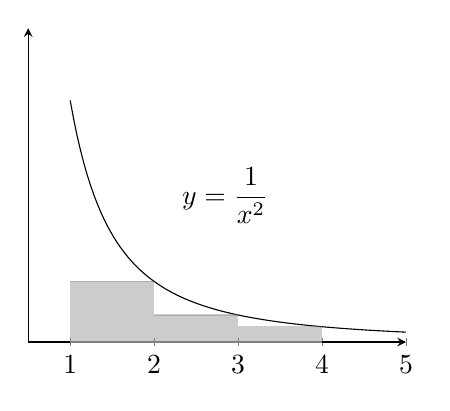
\begin{tikzpicture}[scale=0.7]
        \begin{axis}[
            axis lines = left,
            xmin=0.5,
            ymin=0,
            ymax=1.3,
            ymajorticks=false
        ]
    
        \addplot [domain=1:5, samples=100, color=black,] {(1/x^2) + 0.001} node[above=1cm, pos=0.5] {$\displaystyle y = \frac{1}{x^2}$};
    
        \addplot [domain=1:2,samples=2, color=gray, opacity=0.4, name path=f1,]{0.251};
        \addplot [domain=1:2,samples=2, color=gray, name path=g1,]{0};
        \addplot[gray, opacity=0.4] fill between[of=f1 and g1, soft clip={domain=1:2}];
    
        \addplot [domain=2:3,samples=2, color=gray, opacity=0.4, name path=f2,]{0.1121};
        \addplot [domain=2:3,samples=2, color=gray, name path=g2,]{0};
        \addplot[gray, opacity=0.4] fill between[of=f2 and g2, soft clip={domain=2:3}];
    
        \addplot [domain=3:4,samples=2, color=gray, opacity=0.4, name path=f3,]{0.0635};
        \addplot [domain=3:4,samples=2, color=gray, name path=g3,]{0};
        \addplot[gray, opacity=0.4] fill between[of=f3 and g3, soft clip={domain=3:4}];
        
        \end{axis}
    \end{tikzpicture}
    \caption{Visual interpretation of}
    \text{$\frac{1}{2^2} + \frac{1}{3^2} + \frac{1}{4^2} + \frac{1}{5^2} + \dots$}
    \label{fig:visual series}
\end{minipage}%
\begin{minipage}{.5\textwidth}
      \centering
      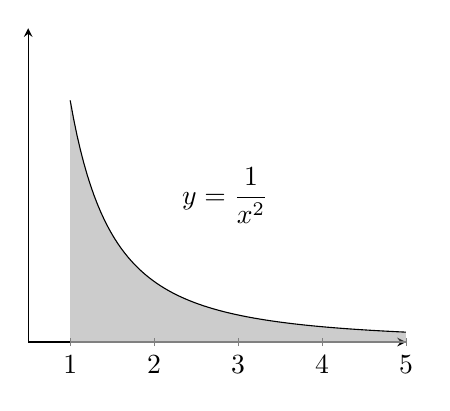
\begin{tikzpicture}[scale=0.7]
        \begin{axis}[
            axis lines = left,
            xmin=0.5,
            ymin=0,
            ymax=1.3,
            ymajorticks=false
        ]
    
        \addplot [domain=1:5, samples=100, color=black, name path=f] {(1/x^2) + 0.001} node[above=1cm, pos=0.5] {$\displaystyle y = \frac{1}{x^2}$};
    
        \addplot [domain=1:5,samples=2, color=gray, name path=g,]{0};

        \addplot[gray, opacity=0.4] fill between[of=f and g, soft clip={domain=1:5}];
        
        \end{axis}
    \end{tikzpicture}
    \caption{Visual interpretation of}
    \text{$\int_{1}^{\infty}\frac{1}{x^2}dx$}
    \label{fig:visual integral}
\end{minipage}
\end{figure}
If we look at equation (\ref{A + B/2 + ...  = ln(infty)}) again and use the fact that everything except $A$ is a constant on the left hand side, we obtain the simpler equation
\begin{equation}
    A = \ln\left(1 + \frac{1}{2} + \frac{1}{3} + \frac{1}{4} + \frac{1}{5} + \dots \right).
\end{equation}
Finally, by using the definition of $A$ and the fact that the Harmonic Series is equal to $\ln(\infty)$ (see equation (\ref{harmonic = ln(infinity)})), Euler obtained
\begin{equation} \label{prime harmonic = ln(ln(infty))}
    \frac{1}{2} + \frac{1}{3} + \frac{1}{5} + \frac{1}{7} + \frac{1}{11} + \dots = \ln(\ln(\infty)).
\end{equation}
For Euler, this was a striking result. Here is what he had to say about this discovery at the beginning of an article he wrote in 1775 called \textit{De summa seriei ex numeris primis formatae [...]} \cite{euler1785summa}:

\begin{quotation}
    Even as Euclid had demonstrated that the multitude of prime numbers is infinite, many years ago I also showed that the sum of the series of the reciprocals of the primes [...] is infinitely large; more precisely, I showed that it has the magnitude of the logarithm of the harmonic series [...] which seems not just a little remarkable, since commonly the harmonic series is counted as the smallest kind of infinite. \footnote{Translated from the Latin by Jordan Bell, Department of Mathematics, University of Toronto, Toronto, Ontario, Canada.}
\end{quotation}

The divergence of the reciprocals of the prime number can be more rigorously stated, with a modern notation, as follows:
\begin{equation}
    \sum_{\substack{p \leq n \\ p \text{ prime}}}\frac{1}{p} = \ln(\ln(n)) + M + o(1)
\end{equation}
where $M$ is a constant called that Meissel-Martens constant. This constant is the analoguous of the Euler constant $\gamma$ for the series of the reciprocals of the prime numbers.

Euler's paper finishes with the proof of the nineteenth theorem. Again, if we forget about rigor, the proof is full of creativity, and it really shows how easy it was for Euler to use all of these seemingly complicated formulas. We often say that Euler's identity:
$$e^{i\pi} + 1 = 0,$$
is beautiful because it links a lot of different concepts in one single equation. However, by looking at Euler's use of logarithms, series, integrals, infinite products, prime numbers, telescoping series, etc \dots, in the previous proof and in his whole paper, it is clear that Euler's identity is, by far, not the only of Euler's work to display such deep links between these different mathematical objects.

At the beginning of this section, I mentionned that the paper we studied would create a link between series of the reciprocals of the powers, and prime numbers. Now that we went over the theorems presented in the paper, we see that this link was established with equation (\ref{Euler Product}). However, for the moment, this link may not seem very surprising. After all, this equation can be interpreted as another way of saying that any natural number can be uniquely written as a product of prime numbers, and that's it. The only original thing about this equation is that it involves series and infinite products. However, this precise equation will turn out to have a great importance in the future of Number Theory. Precisely one century after Euler's Paper, the mathematician Peter Lejeune Dirichlet would use this same equation to prove his famous theorem on arithmetic progressions, and hence, be one of the founder of Analytic Number Theory. 

The second important result of the paper, is equation (\ref{sum of 1/p = infinity}). Again, this result can be interpreted as another way of saying that there are infinitely many primes numbers. What is original about this equation is, again, that it is stated using series, and that it also carries an additional information about the density of the prime number as a subset of the natural numbers. Euler's quote from earlier in this section is from a paper he wrote in 1775 in which he extended his work on the series of the reciprocals of the prime numbers. In this paper, he proved that the series of the reciprocals of the prime numbers of the form $4n+1$ diverges and that the series of the reciprocals of the prime numbers of the form $4n-1$ diverges as well. He even conjectured that the series of the reciprocals of the prime numbers of the form $100n + 1$ diverges. As a direct corollary, we have that there are infinitely many prime numbers of the form $4n+1$ and of the form $4n-1$. These theorems will be extended into a more general theorem proved by Dirichlet: there are infinitely many prime numbers of the form $an + b$ where $a$ and $b$ have no common divisors. Let's end this section with a quote by William Dunham that summerizes well our previous discussion on Euler's work.

\begin{quotation}
    Those familiar with the prime number theorem may forget how wondrous a thing it is, linking primes to the natural logarithm function. Yet this is precisely the sort of connection - between discrete and continuous - that Euler first perceived [...]. If Euler does not quite deserve to be called the "parent" of analytic number theory, let us at least credit him with being its obvious grandparent. \footnote{Quote from the end of Chapter 4, Euler : The Master of Us All \cite{dunham1999euler}. } \\
\end{quotation}

\noindent {\Large\textbf{Exercises}} 

\begin{exercise} \label{Infinite Product convergence}
    The goal of this exercise is to prove that the infinite product $\prod_p (1 - p^{-s})^{-1}$ converges for all real numbers $s > 1$. To prove that it converges, we will mostly rely on properties of the logarithm since it will be used to convert products into a sums. 
    \begin{enumerate}[label=(\alph*)]
        \item Using the Taylor expansion of $\ln(1+x)$, prove that
        $$\ln(1+x) = x + R(x)$$
        for all $x \in (-1, 1)$ where
        $$R(x) = - \frac{x^2}{2}\sum_{n=0}^{\infty}(-1)^n \frac{2x^n}{n+2}.$$ 
        \item Show that $|R(x)| \leq x^2$ when $|x| < 1/2$.
        \item Use part (b) to prove that
        $$|\ln(1+x)| \leq 2|x|$$
        provided $|x| < 1/2$.  
        \item From the inequality proved in part (c), show that the sequence $\prod_{n=1}^{N}(1+a_n)$ converges if we suppose that the series $\sum_{n=1}^{\infty}|a_n|$ converges. Moreover, show that the product converges to 0 only if one of its term is 0.
        \item Conclude that the infinite product $\prod_p (1 - p^{-s})^{-1}$ converges.
    \end{enumerate}
\end{exercise}

\begin{exercise} \label{Euler Product Rigorous Proof}
    The goal of this exercise is to prove Euler's Product Fomula (\ref{Euler Product}) rigorously for all real numbers $s > 1$. If we fix $s > 1$, then by the $p$-series test and Exercise \ref{Infinite Product convergence}, we know that both $\sum_{n=1}^{\infty}n^{-s}$ and $\prod_p (1 - p^{-s})^{-1}$ converge. 
    \begin{enumerate}[label=(\alph*)]
        \item Let $N \leq M$ be two positive integers. Argue that if $n \leq N$ and $n = p_1^{e_1} \cdot ... \cdot p_k^{e_k}$, then $p_i \leq N$ and $e_i \leq M$ for all $i \in \Iint{1}{k}$.
        \item Using part (a), deduce that
        $$\sum_{n=1}^{N}\frac{1}{n^s} \leq \prod_{p \leq N} \sum_{k=1}^{M}\frac{1}{p^{ks}}.$$
        \item Conclude with the following inequality:
        $$\sum_{n=1}^{\infty}\frac{1}{n^s} \leq \prod_p \left(\frac{1}{1 - p^{-s}}\right).$$
        \item To prove the reverse inequality, take positive integers $N$ and $M$ and prove that
        $$\prod_{p \leq N} \sum_{k=1}^{M}\frac{1}{p^{ks}} \leq \sum_{n=1}^{\infty}\frac{1}{n^s}.$$
        \item From part (d), deduce that
        $$\prod_p \left(\frac{1}{1 - p^{-s}}\right) \leq \sum_{n=1}^{\infty}\frac{1}{n^s}$$
        and conclude that the two values are equal.
    \end{enumerate}
\end{exercise}
\section{The Bernoulli Numbers}

As it was mentionned at the end of Section 1.1, Euler really became passionate about series of the form
\begin{equation}\label{series of the reciprocals of the powers of n}
    1 + \frac{1}{2^n} + \frac{1}{3^n} + \frac{1}{4^n} + \frac{1}{5^n} + \dots
\end{equation}
He wrote numerous articles about these series and found several other interesting results other than the ones presented in the two previous sections. In this section, we will study one of these results that Euler found which relates these series with an important sequence of numbers discovered by Jakob Bernoulli. To understand this result, recall that in his 1735 paper, in which he found the value of the series (\ref{series of the reciprocals of the powers of n}) with $n = 2$, he also found a way to deduce all the values of the series (\ref{series of the reciprocals of the powers of n}) where $n$ is an even number. However, even if the method worked really well, it was time consuming since it was recursive: to find the value of the series for some even number $n$, it is required to first find the values of the series for all even numbers smaller than $n$.

A few years later, in his paper \textit{De seriebus quibusdam considerationes} \cite{euler1750seriebus}, written in 1739 and published in 1750, Euler found a better method: a general formula for computing the series (\ref{series of the reciprocals of the powers of n}) which only depends on $n$ when $n$ is even. However, to understand this general formula, we first need to learn about this sequence of the numbers that Jakob Bernoulli found a few decades before.

In his famous book \textit{Ars Conjectandi} \cite{bernoulli1713ars}, published posthumously in 1713, Jakob Bernoulli consider sums of the form
$$1^m + 2^m + 3^m + \dots + n^m.$$
We all have probably seen before that for $m=1$, $m = 2$ and $m=3$, we have the following formulas
\begin{align*}
    1^1 + 2^1 + 3^1 + \dots + n^1 &= \frac{n(n+1)}{2} \\
    1^2 + 2^2 + 3^2 + \dots + n^2 &= \frac{n(n+1)(2n+1)}{6} \\
    1^3 + 2^3 + 3^3 + \dots + n^3 &= \left(\frac{n(n+1)}{2}\right)^2
\end{align*}
which have been known for more than a millenia. With some clever algebraic manipulations, we can find similar formulas for all the higher values of $m$. However, only by looking at the three previous equations, an important question arises: what relates these three formulas ? They have some similarities, but not enough to be able to find their general form (if there is one). It is this question that Bernoulli answered in a chapter of his book.

First, let's rewrite these formulas as well as the formulas for some higher terms of $m$, and let's expand them as polynomials in $n$:
\begin{align*}
    1^0 + 2^0 + 3^0 + \dots + n^0 &= 1\cdot n \\
    1^1 + 2^1 + 3^1 + \dots + n^1 &= \frac{1}{2}n^2 + \frac{1}{2}n \\
    1^2 + 2^2 + 3^2 + \dots + n^2 &= \frac{1}{3}n^3 + \frac{1}{2}n^2 + \frac{1}{6}n \\
    1^3 + 2^3 + 3^3 + \dots + n^3 &= \frac{1}{4}n^4 + \frac{1}{2}n^3 + \frac{1}{4}n^2 + 0\cdot n \\
    1^4 + 2^4 + 3^4 + \dots + n^4 &= \frac{1}{5}n^5 + \frac{1}{2}n^4 + \frac{1}{3}n^3 + 0\cdot n^2 - \frac{1}{30}n \\
    1^5 + 2^5 + 3^5 + \dots + n^5 &= \frac{1}{6}n^6 + \frac{1}{2}n^5 + \frac{5}{12}n^4 + 0\cdot n^3 - \frac{1}{12}n^2 + 0\cdot n
\end{align*}
Written in this way, it seems like there is a lot of patterns to spot: then first term of the sum of the powers of $m$ is always $\frac{n^{m+1}}{m+1}$, the fourth column only contains 0's, the second column only contains $\frac{1}{2}$'s, and so on. But all of these patterns does not let us predict exactly the next formula, the formula for the sum of the $n$ first powers of 6. With our observations, we could guess that this formula might look like
$$1^6 + 2^6 + 3^6 + \dots + n^6 = \frac{1}{7}n^7 + \frac{1}{2}n^6 + An^5 + 0\cdot n^4 + Bn^3 + 0\cdot n^2 + Cn$$
where the coefficients $A$, $B$ and $C$ could not be determined by our observations. Using some pretty complicated algebraic manipulations, we get that the true formula is the following:
$$1^6 + 2^6 + 3^6 + \dots + n^6 = \frac{1}{7}n^7 + \frac{1}{2}n^6 + \frac{1}{2}n^5 + 0\cdot n^4 + -\frac{1}{6}n^3 + 0\cdot n^2 + \frac{1}{42}n$$
which means that we were close. The question now is the following: is there an ultimate pattern that would let us find these formulas easily ? It is exactly this pattern that Bernoulli found and presented in his book.

Without going into the details, the key is to look at the coefficient in front of $n$ in each formula. If we denote by $B_m$ the coefficient in front of $n$ in the formula for the sum of the first $n$ powers of $m$, then using the formulas we displayed above, we get
$$B_0 = 1 \qquad \quad B_1 = \frac{1}{2} \qquad \quad B_2 = \frac{1}{6} \qquad \quad B_3 = 0 \qquad \quad B_4 = -\frac{1}{30} \qquad \quad B_5 = 0$$
These numbers are the first Bernoulli numbers. In general, the $m$th Bernoulli number is the coefficient in front of $n$ in the formula for the sum of the powers of $m$. What Bernoulli noticed is that we only need these numbers to recover all the formulas we found and all the formulas for higher powers. Here is Bernoulli's general formula:
\begin{align*}
    1^m + 2^m + \dots + n^m &= \frac{1}{m+1}\biggl(\frac{1}{1}B_0\cdot n^{m+1} + \frac{m+1}{1}B_1\cdot n^m + \frac{(m+1)m}{1\cdot 2}B_2 \cdot n^{m-1} \\
    &\qquad + \frac{(m+1)m(m-1)}{1\cdot 2\cdot 3}B_3 \cdot n^{m-2} + \dots + (m+1)B_m  \cdot n\biggr)
\end{align*}
This formula looks complicated but if we look at it more closely, we can notice that the coefficients in front of the Bernoulli numbers are simply binomial coefficients. Thus, if we use a more modern notation, we get that Bernoulli's formula becomes
\begin{equation} \label{bernoulli's formula}
    \sum_{i=1}^{n}i^m = \frac{1}{m+1}\sum_{k=0}^{m} \binom{m+1}{k}B_k \cdot n^{m+1-k}
\end{equation}
which now looks a bit simpler. Therefore, thanks to Bernoulli's formula, we get that the problem of finding the formula for the sum of the first $m$th power simply gets reduced to the problem of finding the first $m$ Bernoulli numbers. This seems easier but we quickly run into a problem: we defined and find the Bernoulli numbers by first finding the desired formulas, but we are using the Bernoulli numbers to find these desired formulas, is there another way of finding the Bernoulli numbers without having to find the desired formulas first ? Fortunately, the answer is yes. 

If we plug-in $n = 1$ in equation (\ref{bernoulli's formula}), we obtain the new equation
$$1 = \frac{1}{m+1}\sum_{k=0}^{m}\binom{m+1}{k}B_k$$
which we can rewrite as
\begin{equation}
    B_m = 1 - \sum_{k=0}^{m-1}\binom{m}{k}\frac{B_k}{m-k+1}.
\end{equation}
This equation is precisely what we need since it lets us compute each Bernoulli number using the previous ones. Hence, if we start with the fact that $B_0 = 1$, then this formula lets us compute all Bernoulli numbers. Therefore, the problem of finding a general pattern in the formulas of the sum of the powers of a given positive integer is solved thanks to this mysterious sequence discovered by Jakob Bernoulli. For more informations about the Bernoulli numbers, I strongly recommend the excellent Youtube Video \textit{Power sum MASTER CLASS} \cite{MathologerPowerSum} which is an excellent introduction to the Bernoulli numbers and their applications, such as the Euler-Maclaurin formula. 

We are now ready to go back to Euler's work. Euler was really interested in the sequence formed by the Bernoulli numbers. He found many applications of the Bernoulli numbers, and one of its most remarkable application is the main result of this section. A first very important property of the Bernoulli numbers he found is his summation formula, which is now called the Euler-Maclaurin formula. Without going into the details,  

\td 

\begin{enumerate}
    \item Les nombres de Bernoulli servent a trouver une formula générale pour la somme des entiers d'une puissance donnée. Ce que Euler a découvert c'est que ces memes nombres permettent de trouver une formule générale pour la somme des puissances d'une nombres négatif donné. 
    \item Présenter la démonstration de la formule générale de Euler de son Institutiones.
    \item Remarquer cette formule rend le travail beaucoup plus court.
    \item Remarquer que Euler a étendu le lien entre les nombres de Bernoullis et la somme des puissances positives aux séries de puissances négatives.
    \item Bien qu'Euler soit arrivé aussi loin, toujours rien concernant zeta-3 ou n'importe quel autre valeur impair.
\end{enumerate}

\td 

A first important property of the Bernoulli numbers that Euler found \td [Missing source, might be a good idea to look at Euler's paper on his Euler-Maclaurin formula] \td is the fact that they appear in the series expansion of the function $x/(e^x - 1)$ as follows:
\begin{equation}
    \frac{x}{e^x - 1} = B_0 + \frac{B_1}{1} x + \frac{B_2}{1\cdot 2}x^2 + \frac{B_3}{1\cdot 2 \cdot 3}x^3 + \frac{B_4}{1\cdot \cdot \cdot 4}x^4 + \dots
\end{equation}

\td 

In his book \textit{Institutiones Calculi differentialis} \cite{euler1755institutiones} published in 1755, Euler derives his general formula. I will now present Euler's original proof with some very minor modifications. \td start with produc of sine \td First, he let
\begin{equation}
    V = \frac{u}{1 - e^{-u}} = \frac{(-u)}{e^{(-u)} - 1}.
\end{equation}
Notice that if we plug-in $x = -u$ in equation (\ref{bernoulli numbers definition}), we obtain
\begin{equation} \label{series expansion of V}
    V = B_0 - \frac{B_1}{1}u + \frac{B_2}{1\cdot 2}u^2 - \frac{B_3}{1\cdot 2 \cdot 3}u^3 + \dots = 1 + \frac{1}{2}u + \frac{1}{12}u^2 + \dots
\end{equation}
He then considered the expression
$$V - \frac{1}{2}u = \frac{u}{2} \cdot \frac{1 + e^{-u}}{1 - e^{-u}}$$
and noticed that if we multiply the numerator and the denominator of the righthand side by $e^{-u/2}$, we get
\begin{equation}
    V - \frac{1}{2}u = \frac{u}{2}\cdot \frac{e^{u/2} + e^{-u/2}}{e^{u/2} - e^{-u/2}}.
\end{equation}
Since the expression on the right hand side of the equation remains unchanged after replacing $u$ by $-u$, he concluded that the series expansion must only contain even powers of $u$. It follows from equation (\ref{series expansion of V}) that 
$$V - \frac{1}{2}u = 1 + \frac{B_2}{1\cdot 2}u^2 + \frac{B_4}{1\cdot 2 \cdot 3 \cdot 4}u^4 + ... $$
and so 
\begin{equation} \label{big equation}
    \frac{u}{2}\cdot \frac{e^{u/2} + e^{-u/2}}{e^{u/2} - e^{-u/2}} = 1 + \frac{B_2}{1\cdot 2}u^2 + \frac{B_4}{1\cdot 2 \cdot 3 \cdot 4}u^4 + ... 
\end{equation}
If we replace $u$ by $u\sqrt{-1}$, we get
$$\frac{u}{2} \cdot \frac{\cos(\frac{1}{2}u)}{\sin(\frac{1}{2}u)} = 1 - \frac{B_2}{1\cdot 2}u^2 + \frac{B_4}{1\cdot 2 \cdot 3 \cdot 4}u^4 - ... $$
which we can rewrite as
\begin{equation} \label{expression for cot(u/2)}
    \frac{1}{2}\cot\left(\frac{1}{2}u\right) = \frac{1}{u} - \frac{B_2}{1\cdot 2}u + \frac{B_4}{1\cdot 2 \cdot 3 \cdot 4}u^3 - ...
\end{equation}
Euler proved equation (\ref{expression for cot(u/2)}) from equation (\ref{big equation}) in a different manner but this way is shorter. He then replaced $\frac{1}{2}u$ by $\pi u$ to get
$$\frac{1}{2}\cot(\pi u) = \frac{1}{2\pi u} - \frac{2 \pi B_2}{1\cdot 2}u + \frac{2^3 \pi^3 B_4}{1\cdot 2 \cdot 3 \cdot 4}u^3 - ...$$
By multiplying both sides by $\pi/u$, Euler obtained
$$\frac{\pi}{2u}\cot(\pi u) = \frac{1}{2 u^2} - \frac{2 \pi^2 B_2}{1\cdot 2} + \frac{2^3 \pi^4 B_4}{1\cdot 2 \cdot 3 \cdot 4}u^2 - ...$$
which is equivalent to
\begin{equation}
    \frac{1}{2 u^2} - \frac{\pi}{2u}\cot(\pi u) = \frac{2 \pi^2 B_2}{1\cdot 2} - \frac{2^3 \pi^4 B_4}{1\cdot 2 \cdot 3 \cdot 4}u^2 + ...
\end{equation}
We are halfway done since Euler will now find a second series expansion for $\frac{1}{2 u^2} - \frac{\pi}{2u}\cot(\pi u)$ and equate the two expansions he found to obtain his general formula. To do so, Euler started this time from the product formula of the function $\sin(\pi x)$ \td 

\td 
\section{The Odd Number Problem}

It seems like there is not much left to be discovered for Euler. He not only solved the Basel Problem, but solved it for all even numbers (\autoref{sec: Basel Problem}), created a link between these series and the prime numbers (\autoref{sec: prime numbers}), and even found a link between the values of these series and the coefficients of the formula he used in the first place to approximate these numbers (\autoref{sec:summation formula} and \autoref{sec: bernoulli numbers}). But looking back at these results, there is one clear missing piece: what is the value of the series
$$1 + \frac{1}{2^n} + \frac{1}{3^n} + \frac{1}{4^n} + \frac{1}{5^n} + \dots$$
when $n$ is an odd number ? Since the very begining of Euler's work on these series, he tried solving this problem. In \autoref{sec:summation formula}, he approximated the series of the reciprocals of the squares very precisely but also did the same for the series of the reciprocals of the cubes:
$$1 + \frac{1}{2^3} + \frac{1}{3^3} + \frac{1}{4^3} + \frac{1}{5^3}+ \dots = 1.202056903159594$$
When solving the Basel Problem in \autoref{sec: Basel Problem}, he solved it for all even powers of $n$ with one general and powerful trick which turned out to be ineffective for odd values of $n$. He was still able to obtain the following series:
$$1 - \frac{1}{3^3} + \frac{1}{5^3} - \frac{1}{7^3} + \frac{1}{9^3} - \dots = \frac{\pi^3}{32}.$$
When establishing his product formula (\ref{Euler Product}) in \autoref{sec: prime numbers}, Euler obtained the equation
$$1 + \frac{1}{2^3} + \frac{1}{3^3} + \frac{1}{4^3} + \frac{1}{5^3}+ \dots = \frac{2^3}{2^3 - 1}\cdot \frac{3^3}{3^3 - 1}\cdot\frac{5^3}{5^3 - 1}\cdot\frac{7^3}{7^3 - 1}\cdot\cdot\cdot$$
which is not useful for finding the exact value of the series of the reciprocals of the cubes. Finally, when discovering that the Bernoulli numbers encode the values of the series associated with even values of $n$ in \autoref{sec: bernoulli numbers}, he was unable to generalize this result since he proved himself that the Bernoulli numbers are zero for all odd values of $n \geq 3$. In each of the articles containing these results, Euler always mentions that unfortunately, none of his efforts were able to lead him to the value of the series where $n$ is odd.

Euler attempted to find the value of the series of the reciprocals of the cubes way more times than just the ones presented above. For example, in his 44 pages long article \textit{De seriebus quibusdam considerationes} \cite{eulerE130}, written in 1739 and published in 1750, Euler tries everything he can to find the value of this series. This article contains most of Euler's results presented in \autoref{sec: bernoulli numbers}, but at that time, Euler didn't notice that the numbers he was studying were the Bernoulli numbers. In the article, Euler manages to find many surprising equivalent expressions of the sum of the reciprocals of the cubes such as the following one:
\begin{align*}
    1 + \frac{1}{2^3} + \frac{1}{3^3} + \frac{1}{4^3} + \dots = \frac{\pi^2}{6}\ln(2) & - \frac{1}{2^2}\left(\frac{1}{2\cdot 2}\right) \\
    &-\frac{1}{3^2}\left(\frac{1}{2\cdot 2} + \frac{1 \cdot 3}{2 \cdot 4 \cdot 4}\right) \\ 
    &-\frac{1}{4^2}\left(\frac{1}{2\cdot 2} + \frac{1 \cdot 3}{2 \cdot 4 \cdot 4} + \frac{1 \cdot 3 \cdot 5}{2 \cdot 4 \cdot 6 \cdot 6}\right) \\ 
    &-\frac{1}{5^2}\left(\frac{1}{2\cdot 2} + \frac{1 \cdot 3}{2 \cdot 4 \cdot 4} + \frac{1 \cdot 3 \cdot 5}{2 \cdot 4 \cdot 6 \cdot 6} + \frac{1 \cdot 3 \cdot 5 \cdot 7}{2 \cdot 4 \cdot 6 \cdot 8 \cdot 8}\right) \\
    & \quad etc...
\end{align*}
However, despite all of his efforts, the article ends with the following (very sad) paragraph which probably captures Euler's feeling after searching this value for 10 years.

\begin{quote}
    But because, no matter how we transform this series, we are not able to reduce it to a simple series, whose sum is known, we stop our attempts here, contented by these many expressions equivalent to the propounded series $1 - \frac{1}{2^3} + \frac{1}{3^2} - \frac{1}{4^3} + \frac{1}{5^2} - etc.$ \footnote{This translation was made by Alexander Aycock.}
\end{quote}
However, this was not Euler's final attempt, there is another attempt that really deserves our attention. In his article \textit{Remarques sur un beau rapport entre les séries des puissances tant directes que réciproques} \cite{eulerE353}, written in 1749 and published in 1768, Euler finds a curious formula which will turn out to have a great importance in the study of L-functions. Let's take a look at this article.

\subsection*{On Divergent Series}

First, let's recall that the alternating and non-alternating series of the reciprocals of the $n$th powers are related by this equation:
\begin{equation} \label{direct sum in terms of alterne}
    1 + \frac{1}{2^n} + \frac{1}{3^n} + \frac{1}{4^n} + \dots = \frac{2^{n-1}}{2^{n-1} - 1}\left(1 - \frac{1}{2^n} + \frac{1}{3^n} - \frac{1}{4^n} + \dots\right).
\end{equation}
Therefore, finding the series on the left hand side is equivalent to finding the series on the right hand side. This explains why Euler will study series of the following form in his article:
$$\frac{1}{1^n} - \frac{1}{2^n} + \frac{1}{3^n} - \frac{1}{4^n} + \frac{1}{5^n} - \frac{1}{6^n} + \dots$$
which he will call series of the \textit{first species}. Curiously, he will then define series of the \textit{second species} to be the series of the form 
$$1^n - 2^n + 3^n - 4^n + 5^n - 6^n + \dots$$
This is surprising because the series of the second species are obviously divergent (assuming $n$ to be positive). But Euler didn't simply assume that these series could be manipulated as if they were convergent, he knew that it would lead to some contradictions. In his article \textit{De seriebus divergentibus} \cite{eulerE247} written in 1746 and published in 1760, the first 12 sections are precisely dedicated to making sense of diverging series and the values that can be assigned to these series. Without going into the details of this paper, Euler's conclusion is that the sum of a series can be defined as the finite expression from which the series is generated. For example, since the series
$$1 + x + x^2 + x^3 + x^4 + x^5 + \dots$$
is generated by the finite expression
$$\frac{1}{1-x},$$
then by plugging-in $x = -1$, Euler concluded that
$$1 - 1 + 1 - 1 + 1 - 1 + \dots = \frac{1}{2}.$$
However, he also raised an important matter: by plugging-in $x = 2$, he obtained
$$1 + 2 + 4 + 8 + 16 + 32 + \dots = -1$$
which seems to contradict the laws of mathematics since one can never obtain a negative value by adding positive quantities. He mentioned that some mathematicians made sense of this using the following argument: the sequence
$$\frac{1}{4}, \quad \frac{1}{3}, \quad \frac{1}{2}, \quad \frac{1}{1}, \quad \frac{1}{0}, \quad \frac{1}{-1}, \quad \frac{1}{-2}, \quad \frac{1}{-3}, \quad \frac{1}{-4}, \quad etc$$
has increasing positive terms and also increasing negative terms, and so if this sequence is seen as being increasing, then we obtain the inequality $-\frac{1}{2} > \infty$ which explains the equation above. Thus, the negative numbers would be the numbers greater than $\infty$ and smaller than $0$ while the positive numbers are the numbers greater than 0 and smaller than $\infty$. Visually, this means that we can visualize the real numbers not as an infinite straight line but as a circle (\autoref{fig: circle representation}).
\begin{figure}[h!]
\centering
\begin{tikzpicture}
    \draw[fill=none](0,0) circle (1.2) node [black,yshift=-2cm] {};
    \draw[fill=black](1.2,0) circle (1 pt) node [right] {1};
    \draw[fill=black](0,1.2) circle (1 pt) node [above] {$\infty$};
    \draw[fill=black](-1.2,0) circle (1 pt) node [left] {-1};
    \draw[fill=black](0,-1.2) circle (1 pt) node [below] {0};
\end{tikzpicture}
\caption{Circle representation of the real numbers}
\label{fig: circle representation}
\end{figure}
But Euler rejected this argument since, according to him, it would imply that $-1$ behaves differently if it is obatined as $(a+1) - a$ or as $\frac{1}{-1}$. Therefore, Euler would only consider alternating diverging series to avoid these difficulties. This also explains why Euler focuses on alternating series in his 1749 article.

Returning to the main article, Euler considered the equation
$$1 - x + x^2 - x^3 + x^4 - x^5 + \dots = \frac{1}{1+x},$$
from which he obtained the following ones by successively multiplying both sides by $x$ and taking the derivative:
\begin{align*}
    1 - x + x^2 - x^3 + \dots &= \frac{1}{1+x}, \\
    1 - 2x + 3x^2 - 4x^3 + \dots &= \frac{1}{(1+x)^2}, \\
    1 - 2^2x + 3^2x^2 - 4^2x^3 + \dots &= \frac{1-x}{(1+x)^3}, \\
    1 - 2^3x + 3^3x^2 - 4^3x^3 + \dots &= \frac{1-4x + x^2}{(1+x)^4}, \\
    1 - 2^4x + 3^4x^2 - 4^4x^3 + \dots &= \frac{1 - 11x + 11x^2 - x^3}{(1+x)^5}, \\
    1 - 2^5x + 3^5x^2 - 4^5x^3 + \dots &= \frac{1 - 26x + 66x^2 - 26x^3 + x^4}{(1+x)^6}.
\end{align*}
Hence, by his study of diverging series, he obtained the following values for the series of the second species by taking $x = 1$:
\begin{align*}
    1 - 2^0 + 3^0 - 4^0 + 5^0 - 6^0 + \dots &= \frac{1}{2}, \\
    1 - 2^1 + 3^1 - 4^1 + 5^1 - 6^1 + \dots &= \frac{1}{4}, \\
    1 - 2^2 + 3^2 - 4^2 + 5^2 - 6^2 + \dots &= 0, \\
    1 - 2^3 + 3^3 - 4^3 + 5^3 - 6^3 + \dots &= -\frac{2}{16}, \\
    1 - 2^4 + 3^4 - 4^4 + 5^4 - 6^4 + \dots &= 0, \\
    1 - 2^5 + 3^5 - 4^5 + 5^5 - 6^5 + \dots &= +\frac{16}{64}, \\
    1 - 2^6 + 3^6 - 4^6 + 5^6 - 6^6 + \dots &= 0, \\
    1 - 2^7 + 3^7 - 4^7 + 5^7 - 6^7 + \dots &= -\frac{272}{256}.
\end{align*}
By looking at these values, we can clearly recognize the pattern of the Bernoulli numbers in the signs and the zeros of the sequence generated by these values. But to prove this, Euler would have to use his summation formula (\autoref{sec:summation formula}) in a new way.

\subsection*{The Infinite Summation Formula}

Recall that at first, Euler's summation formula was developed to interpolate the sequence of partial sums of a general function. In other words, it interpolates the function defined by
$$f(a) + f(a + b) + f(a + 2b) + f(a + 3b) + \dots + f(x)$$
where $a$ and $b$ are two numbers ($b$ is assumed to be positive). However, Euler would now focus on a new problem: extending the function
$$f(x) - f(x + a) + f(x + 2) - f(x + 3) + f(x + 4) - \dots$$
where the sum is infinite. This time, the variable $x$ is not related to the number of terms in the summation but indicates the value of the first index. This seemingly distinct problem will turn out to be really similar to the original one.

First, Euler would let
$$S(x) = f(x) + f(x + a) + f(x + 2) + f(x + 3) + \dots$$
and use Taylor's formula (Equation (\ref{Taylor's Formula})) to obtain 
$$S(x+a) = S(x) + \frac{adS}{1dx} + \frac{a^2 ddS}{1\cdot 2 dx^2} + \frac{a^3 d^3S}{1\cdot 2\cdot 3 dx^3} + \frac{a^4 d^4S}{1\cdot 2\cdot 3 \cdot 4 dx^4} + \dots$$
from which he obtained 
\begin{equation} \label{-f = sum}
    -f(x) = \frac{adS}{1dx} + \frac{a^2 ddS}{1\cdot 2 dx^2} + \frac{a^3 d^3S}{1\cdot 2\cdot 3 dx^3} + \frac{a^4 d^4S}{1\cdot 2\cdot 3 \cdot 4 dx^4} + \dots
\end{equation}
by using the fact that $S(x+a) - S(x) = -f(x)$ from the  definition of $S(x)$. Next, in view of inverting equation (\ref{-f = sum}), he wrote
\begin{equation}\label{ds/dx in terms of c_ns}
    \frac{dS}{dx} = c_0 f(x) + c_1 \frac{df}{dx} + c_2 \frac{d^2 f}{dx^2} + c_3 \frac{d^3 f}{dx^3} +\dots
\end{equation}
By plugging the previous equation into equation (\ref{-f = sum}), he obtained
\begin{align*}
    -f(x) &= \frac{a}{1}\left(c_0 f(x) + c_1 \frac{df}{dx} + c_2 \frac{d^2f}{dx^2} + c_3 \frac{d^3f}{dx^3} +  + \dots\right) \\
    &+\frac{a^2}{2}\left(c_0 \frac{df}{dx} + c_1 \frac{d^2f}{dx^2} + c_2 \frac{d^3f}{dx^3} + \dots\right) \\
    &+ \frac{a^3}{6}\left(c_0 \frac{d^2f}{dx^2} + c_1 \frac{d^3f}{dx^3} + \dots\right) \\
    &+ \frac{a^4}{24}\left(c_0 \frac{d^3f}{dx^3} + \dots\right)
\end{align*}
which he rewrote as 
\begin{align*}
    -f(x) &= \frac{ac_0}{1} f(x) \\
    &+ \left(\frac{ac_1}{1} + \frac{a^2c_0}{2}\right)\frac{df}{dx} \\
    &+ \left(\frac{ac_2}{1} + \frac{a^2c_1}{2} + \frac{a^3 c_0}{6} \right)\frac{d^2f}{dx^2}  \\
    &+ \left(\frac{ac_3}{1} + \frac{a^2c_2}{2} + \frac{a^3 c_1}{6} + \frac{a^4 c_0}{24}\right)\frac{d^3f}{dx^3} \\
    &+ \dots 
\end{align*}
Next, by comparing the coefficients in front of the derivatives of $f$ on both sides, Euler obtained the following equations:
\begin{align*}
    c_0 &= -\frac{1}{a} \\
    c_1 &= -\frac{ac_0}{2} \\
    c_2 &= -\frac{ac_1}{2} - \frac{a^2c_0}{6} \\
    c_3 &= -\frac{ac_2}{2} - \frac{a^2c_1}{6} - \frac{a^3c_0}{24}
\end{align*}
which he used to get
$$c_0 = -\frac{1}{a}, \qquad c_1 = \frac{1}{2}, \qquad c_2 = -\frac{a}{12}, \qquad c_3 = 0, \qquad c_4 = \frac{a^4}{720}, \qquad c_5 =0, \quad etc ...$$
Then, Euler noticed that the sequence of $c_n$'s could be written in terms of the sequence of $\alpha_n$'s found for its original summation formula (\autoref{sec:summation formula}): $c_n = (-a)^{n-1}\alpha_n$ for all $n \geq 0$ (Exercise \ref{ex: c_n generating function}). Thus, plugging everything in equation (\ref{ds/dx in terms of c_ns}) and integrating both sides gives:
$$f(x) + f(x + a) + f(x + 2a) + f(x + 3a) + \dots$$
$$= - \frac{\alpha_0}{a}\int f(x) dx + \alpha_1f(x) - \frac{a\alpha_2 df}{dx} + \frac{a^2 \alpha_3 d^2f}{dx^2} - \frac{a^3 \alpha_4 d^3f}{dx^3} + \dots$$
From this equation, Euler replaced $a$ with $2a$ and multiplied both sides by $2$ to obtain
$$2f(x) + 2f(x + 2a) + 2f(x + 4a) + 2f(x + 6a) + \dots$$
$$= - \frac{\alpha_0}{a}\int f(x) dx + 2\alpha_1f(x) - \frac{2^2a\alpha_2 df}{dx} + \frac{2^3a^2 \alpha_3 d^2f}{dx^2} - \frac{2^4a^3 \alpha_4 d^3f}{dx^3} + \dots$$
Finally, he subtracted from this equation the one above to obtain the desired formula:
\begin{center}
$$f(x) - f(x + a) + f(x + 2a) - f(x + 3a) + \dots$$
$$= \alpha_1f(x) - \frac{(2^2-1)a\alpha_2 df}{dx} + \frac{(2^3-1)a^2 \alpha_3 d^2f}{dx^2} - \frac{(2^4-1)a^3 \alpha_4 d^3f}{dx^3} + \dots$$
\end{center}
From this general formula, he considered the special case where $f(x) = x^m$ and $a = 1$:
$$x^m - (x + 1)^m + (x + 2)^m - (x + 3)^m + \dots$$
$$= \alpha_1x^m - m(2^2-1)\alpha_2x^{m-1} + m(m-1)(2^3-1) \alpha_3x^{m-2} - m(m-1)(m-2)(2^4-1) \alpha_4 x^{m-3} + \dots$$
Notice that the series at the bottom in the above equation has finitely many terms since all the terms will vanish after the first $m+1$ terms. To get the values of the series of the second species, Euler noticed that instead of plugging $x = 1$, it is more convenient and way easier to plug-in $x = 0$ since the series becomes
$$0^m - 1^m + 2^m - 3^m + 4^m - 5^m + \dots$$
and only the constant term in the bottom polynomial will be non-zero. From these observations and by multiplying both sides of the equation by $-1$ when $m > 0$, Euler obtained the following values
\begin{align*}
    1 - 2^0 + 3^0 - 4^0 + 5^0 - 6^0 + \dots &= \alpha_1, \\
    1 - 2^1 + 3^1 - 4^1 + 5^1 - 6^1 + \dots &= +1\cdot(2^2-1)\alpha_2, \\
    1 - 2^2 + 3^2 - 4^2 + 5^2 - 6^2 + \dots &= -1\cdot 2\cdot (2^3-1) \alpha_3, \\
    1 - 2^3 + 3^3 - 4^3 + 5^3 - 6^3 + \dots &= +1\cdot 2 \cdot 3\cdot (2^4-1) \alpha_4, \\
    1 - 2^4 + 3^4 - 4^4 + 5^4 - 6^4 + \dots &= -1\cdot 2 \cdot 3\cdot 4 \cdot (2^5-1) \alpha_5, \\
    1 - 2^5 + 3^5 - 4^5 + 5^5 - 6^5 + \dots &= +1\cdot 2 \cdot 3\cdot 4 \cdot 5 \cdot  (2^6-1) \alpha_6, \\
    1 - 2^6 + 3^6 - 4^6 + 5^6 - 6^6 + \dots &= -1\cdot 2 \cdot 3\cdot 4 \cdot 5 \cdot 6 \cdot (2^7-1) \alpha_7, \\
    1 - 2^7 + 3^7 - 4^7 + 5^7 - 6^7 + \dots &= +1\cdot 2 \cdot 3\cdot 4 \cdot 5 \cdot 6 \cdot 7 \cdot (2^8-1) \alpha_8
\end{align*}
which are consistent with the values found above. Using the fact that $\alpha_{n} = 0$ for all odd integers $n \geq 3$, we can remove the minus signs on the right hand side of the previous equations to obtain
\begin{align*}
    1 - 2^0 + 3^0 - 4^0 + 5^0 - 6^0 + \dots &= 1\cdot(2^1 - 1)\alpha_1, \\
    1 - 2^1 + 3^1 - 4^1 + 5^1 - 6^1 + \dots &= 1\cdot(2^2-1)\alpha_2, \\
    1 - 2^2 + 3^2 - 4^2 + 5^2 - 6^2 + \dots &= 1\cdot 2\cdot (2^3-1) \alpha_3, \\
    1 - 2^3 + 3^3 - 4^3 + 5^3 - 6^3 + \dots &= 1\cdot 2 \cdot 3\cdot (2^4-1) \alpha_4, \\
    1 - 2^4 + 3^4 - 4^4 + 5^4 - 6^4 + \dots &= 1\cdot 2 \cdot 3\cdot 4 \cdot (2^5-1) \alpha_5, \\
    1 - 2^5 + 3^5 - 4^5 + 5^5 - 6^5 + \dots &= 1\cdot 2 \cdot 3\cdot 4 \cdot 5 \cdot  (2^6-1) \alpha_6, \\
    1 - 2^6 + 3^6 - 4^6 + 5^6 - 6^6 + \dots &= 1\cdot 2 \cdot 3\cdot 4 \cdot 5 \cdot 6 \cdot (2^7-1) \alpha_7, \\
    1 - 2^7 + 3^7 - 4^7 + 5^7 - 6^7 + \dots &= 1\cdot 2 \cdot 3\cdot 4 \cdot 5 \cdot 6 \cdot 7 \cdot (2^8-1) \alpha_8
\end{align*}
which makes the pattern even clearer. Using a modern notation, we can rewrite these equations as follows:
\begin{equation} \label{alternate negative values}
    \sum_{n=1}^{\infty}(-1)^{n+1}n^m = m!(2^{m+1} - 1)\alpha_{m+1}.
\end{equation}
Therefore, using his infinite summation formula, Euler was able to find the general formula for the series of the second species. Again, this general formula involves the $\alpha_n$'s which are closely related to the Bernoulli numbers. 

\subsection*{A Curious Ratio Between Two Series}

Euler recalled the general formula for the series of the first species he found before (\autoref{sec: bernoulli numbers}) which also involves the $\alpha_n$'s:
\begin{align*}
    1 + \frac{1}{2^2} + \frac{1}{3^2} + \frac{1}{4^2} + \dots &= +2 \alpha_2 \pi^2 \\
    1 + \frac{1}{2^4} + \frac{1}{3^4} + \frac{1}{4^4} + \dots &= -2^3 \alpha_4 \pi^4 \\
    1 + \frac{1}{2^6} + \frac{1}{3^6} + \frac{1}{4^6} + \dots &= +2^5 \alpha_6 \pi^6 \\
    1 + \frac{1}{2^8} + \frac{1}{3^8} + \frac{1}{4^8} + \dots &= - 2^7 \alpha_8 \pi^8
\end{align*}
Then, using the fact that $\alpha_n = 0$ for all odd integers $n \geq 3$ and the fact that the sum
$$\frac{1}{1^n} + \frac{1}{2^n} + \frac{1}{3^n} + \frac{1}{4^n} + ...$$
is nonzero for all positive integers $n$, he obtained the following ratios by dividing the series of the second species by the corresponding series of the first species:
\begin{align*}
  \frac{1 \; - \; 2 \; + \; 3 \;- \; 4 \; + \; 5 \,  - \;  6 \; + \&c.}{\displaystyle 1 - \frac{1}{2^2} + \frac{1}{3^2} - \frac{1}{4^2} + \frac{1}{5^2} - \frac{1}{6^2} + \&c.} &= + \frac{1(2^2-1)}{(2-1)\pi^2} \\
  \frac{1 - \, 2^2 + \, 3^2- \, 4^2 + \, 5^2  - \,  6^2 + \&c.}{\displaystyle 1 - \frac{1}{2^3} + \frac{1}{3^3} - \frac{1}{4^3} + \frac{1}{5^3} - \frac{1}{6^3} + \&c.} &= 0 \\
  \frac{1 - \, 2^3 + \, 3^3- \, 4^3 + \, 5^3  - \,  6^3 + \&c.}{\displaystyle 1 - \frac{1}{2^4} + \frac{1}{3^4} - \frac{1}{4^4} + \frac{1}{5^4} - \frac{1}{6^4} + \&c.} &= - \frac{1\cdot 2 \cdot 3(2^4 - 1)}{(2^3 - 1)\pi^4} \\
  \frac{1 - \, 2^4 + \, 3^4- \, 4^4 + \, 5^4  - \,  6^4 + \&c.}{\displaystyle 1 - \frac{1}{2^5} + \frac{1}{3^5} - \frac{1}{4^5} + \frac{1}{5^5} - \frac{1}{6^5} + \&c.} &= 0 \\
  \frac{1 - \, 2^5 + \, 3^5- \, 4^5 + \, 5^5  - \,  6^5 + \&c.}{\displaystyle 1 - \frac{1}{2^6} + \frac{1}{3^6} - \frac{1}{4^6} + \frac{1}{5^6} - \frac{1}{6^6} + \&c.} &= + \frac{1\cdot 2 \cdot \cdot 5(2^6 - 1)}{(2^5 - 1)\pi^6}
\end{align*}
in which the $\alpha_n$'s cancel out. From this, Euler rewrote these equations in the following single formula:
\begin{equation} \label{curious ratio}
    \boxed{\frac{1 - 2^{n-1} + 3^{n-1} - 4^{n-1}+ ...}{\displaystyle 1 \, - \, \frac{1}{2^n} \ + \: \frac{1}{3^n} \ - \: \frac{1}{4^n} \ + ...} = \frac{-1\cdot 2 \cdot \cdot \cdot (n-1)(2^n - 1)}{(2^{n-1} - 1)\pi^n}\cos \left(\frac{n \pi }{2}\right)}
\end{equation}
for all integers $n \geq 2$. This formula seems strange but it is really just a mix between the two general formulas Euler found before. Moreover, the additional cosine factor is just here to make the signs alternate and be equal to $0$ when $n$ is odd. However, Euler's surprising observation is that equation (\ref{curious ratio}) is true not just for the integers $n \geq 2$ but for all values of $n$ (in the sense that it holds for all real numbers $n$). This is surprising because for $n = 1$, we know from earlier that
\begin{align*}
    1 - 1 + 1 - 1 + 1 - 1 + ... &= \frac{1}{2} \\
    1 - \frac{1}{2} + \frac{1}{3} - \frac{1}{4} + \frac{1}{5} - \frac{1}{6} + \dots &= \ln 2
\end{align*}
and so the left hand side of equation (\ref{curious ratio}) becomes
$$\frac{1 - 1 + 1 - 1 + 1 - 1 + ...}{\displaystyle 1 - \frac{1}{2} + \frac{1}{3} - \frac{1}{4} + \frac{1}{5} - \frac{1}{6} + \dots} = \frac{1}{2\ln 2}$$
which seems to contradict Euler's observation since the right hand of the equation involves no natural logarithm. When evaluating the right hand side of equation (\ref{curious ratio}) at $n = 1$, we get that $1\cdot 2 \cdot \cdot \cdot (n-1) = 1$ (since $0! = 1$), $2^n - 1 = 1$ and so we are only left with $-1/\pi$ multiplied by
$$\frac{\cos\left(\frac{n\pi}{2}\right)}{2^{n-1} - 1}$$
in which both the numerator and the denominator vanish. Euler then considered the variable $n$ to be continuous and stated that this ratio is equal to the ratio of the differentials of the numerator and denominator (which is now known as l'Hopital's Rule). Since the differential of the numerator is $-\frac{\pi dn}{2}\sin(\frac{n\pi}{2})$ and the differential of the denominator is $2^{n-1}dn \ln 2$, then at $n = 1$ we obtain
$$-\frac{1}{\pi}\frac{\cos\left(\frac{n\pi}{2}\right)}{2^{n-1} - 1} = -\frac{1}{\pi}\frac{-\frac{\pi}{2}\sin(\frac{n\pi}{2})}{2^{n-1}\ln 2} = \frac{1}{2\ln 2}.$$
Therefore, Euler proved that his formula holds for the case $n = 1$. In a similar way, he also proved that it also holds for the case $n = 0$ (Exercise \ref{ex: curious ratio n=0}).

For Euler, proving that the formula holds for all integers $n \geq 2$, as well as for the non-trivial cases $n = 0$ and $n = 1$ is already a strong proof that his observation is true since, as he said in his article, it seems impossible for a false supposition to lead to such proofs. But even after these proofs, he was still willing to give more proofs that his observation is true. Here, it is important to notice that during Euler's time, a proof was simply an argument in favor of a conjecture. Thus, from Euler's point of view, he already gave two proofs of his observation with the cases $n = 0$ and $n = 1$.

To make his formula even more certain, Euler then proved that it also holds for the negative integers. To do so, he let $n$ be a negative integer and defined the positive integer $m = -(n - 1)$. Since the formula holds for the integer $m$, then we have
$$\frac{1 - 2^{-n} + 3^{-n} - 4^{-n}+ ...}{\displaystyle 1 - 2^{n-1} +  3^{n-1} - 4^{n-1}  + ...} = \frac{-1\cdot 2 \cdot \cdot \cdot (-n)(2^{1-n} - 1)}{(2^{-n} - 1)\pi^{1-n}}\cos \left(\frac{(1-n) \pi }{2}\right).$$
Next, Euler denoted by $[\lambda]$ the product $1 \cdot 2 \cdot 3 \cdot \cdot \cdot \lambda$ (which we now denote by $\lambda !$) and recalled the following formula which he proved before:
\begin{equation} \label{euler sin factorial}
    [\lambda][-\lambda] = \frac{\pi \lambda}{\sin(\pi \lambda)}.
\end{equation}
This formula is strange since the product $1 \cdot 2 \cdot 3 \cdot \cdot \cdot (-\lambda)$ doesn't intuitively make sense when $\lambda$ is a positive integer. However, a few years before this paper, Euler was able to interpolate the function $[\lambda]$ so that $\lambda$ can be any number, not just the positive integers. Therefore, equation (\ref{euler sin factorial}) is valid in the sense of Euler's interpolation. More informations about interpolations of the function $[\lambda]$ in \autoref{chap:GammaFunction}.

In equation (\ref{euler sin factorial}), Euler took $\lambda = n$ to obtain
$$1\cdot 2 \cdot 3 \cdot \cdot \cdot (-n) = [-n] = \frac{\pi n}{[n] \sin(\pi n)} = \frac{\pi}{1\cdot 2 \cdot \cdot \cdot (n-1) \sin(\pi n)}$$
which he substituted in the equation above to get
$$\frac{1 - 2^{-n} + 3^{-n} - 4^{-n}+ ...}{\displaystyle 1 - 2^{n-1} +  3^{n-1} - 4^{n-1}  + ...} = -\frac{(2^{1-n} - 1)\pi^n}{1\cdot 2 \cdot \cdot \cdot (n - 1)(2^{-n} - 1)\sin(\pi n)}\sin \left(\frac{n\pi }{2}\right)$$
using the fact that $\cos(\frac{(1-n)\pi}{2}) = \sin(\frac{n\pi}{2})$. Then, he simplified the expression on the right hand side by multiplying the numerator and the denominator by $2^n$ and by using the fact that $2 \sin(\frac{n\pi}{2})\cos(\frac{n\pi}{2}) = \sin(n\pi)$ to obtain
$$\frac{1 - 2^{-n} + 3^{-n} - 4^{-n}+ ...}{\displaystyle 1 - 2^{n-1} +  3^{n-1} - 4^{n-1}  + ...} = -\frac{(2^{n-1} - 1)\pi^n}{1\cdot 2 \cdot \cdot \cdot (n - 1)(2^{n} - 1)\cos \left(\frac{n\pi }{2}\right)}.$$
Finally, taking the inverse on both sides gives the equation 
$$\frac{\displaystyle 1 - 2^{n-1} +  3^{n-1} - 4^{n-1}  + ...}{1 - 2^{-n} + 3^{-n} - 4^{-n}+ ...} = \frac{-1\cdot 2 \cdot \cdot \cdot (n - 1)(2^{n} - 1)}{(2^{n-1} - 1)\pi^n}\cos \left(\frac{n\pi }{2}\right)$$
which is precisely the desired result. Therefore, the formula is true for all (positive and negative) integers. 

But there is still one last case that Euler considered: the case $n = \frac{1}{2}$. If we plug-in this value of $n$ in the left hand side of equation (\ref{curious ratio}), we get
$$\frac{1 - \frac{1}{\sqrt{2}} + \frac{1}{\sqrt{3}} - \frac{1}{\sqrt{4}} + \frac{1}{\sqrt{5}} - \frac{1}{\sqrt{6}} + ...}{1 - \frac{1}{\sqrt{2}} + \frac{1}{\sqrt{3}} - \frac{1}{\sqrt{4}} + \frac{1}{\sqrt{5}} - \frac{1}{\sqrt{6}} + ...} = 1.$$
For the right hand side of the equation, we obtain
$$\frac{-1\cdot 2 \cdot \cdot \cdot (n - 1)(2^{n} - 1)}{(2^{n-1} - 1)\pi^n}\cos \left(\frac{n\pi }{2}\right) = -\frac{[-\frac{1}{2}](\sqrt{2} - 1)}{(\frac{1}{\sqrt{2}} - 1)\sqrt{\pi}}\cos \left(\frac{\pi }{4}\right) = \frac{[-\frac{1}{2}]}{\sqrt{\pi}} = 1$$
where the last equality comes from the fact that Euler proved before that $[-\frac{1}{2}] = \sqrt{\pi}$ (\autoref{chap:GammaFunction}). Therefore, both sides of equation (\ref{curious ratio}) are still equal if we replace $n$ with $\frac{1}{2}$. Hence, for Euler, the formula is now true with \textit{the highest degree of certainty} (using his words) since it holds not only for the integers but also for some fractions.

\subsection*{The Odd Powers}

But Euler didn't end his paper on these proofs, he used his brand new formula to attack the original probem of finding the sum of the reciprocals of the integers raised to an odd power. As we have seen earlier (equation (\ref{direct sum in terms of alterne})), this problem is equivalent to finding the value of the series
$$1 - \frac{1}{2^n} + \frac{1}{3^n} - \frac{1}{4^n} + \frac{1}{5^n} - \frac{1}{6^n} + ...$$
where $n$ is an odd number. Thus, he rewrote his ratio formula as follows:
$$1 - \frac{1}{2^{2\lambda + 1}} + \frac{1}{3^{2\lambda + 1}} - \frac{1}{4^{2\lambda + 1}} + \dots $$
$$= \frac{(2^{2\lambda} - 1)\pi^{2\lambda + 1}}{-1\cdot 2 \cdot \cdot \cdot (2\lambda)(2^{2\lambda + 1} - 1)} \cdot \frac{1 - 2^{2\lambda} + 3^{2\lambda} - 4^{2\lambda}+ ...}{\cos(\frac{(2\lambda + 1)\pi}{2})}.$$
However, he quickly made the observation that both the numerator and the denominator of the second factor on the bottom of the previous equation are zero. Therefore, after substituting this ratio with the ratio of the respective differentials (l'Hopital's Rule), he obtained 
$$1 - \frac{1}{2^{2\lambda + 1}} + \frac{1}{3^{2\lambda + 1}} - \frac{1}{4^{2\lambda + 1}} + \dots$$
$$= \frac{2(2^{2\lambda} - 1)\pi^{2\lambda}}{1\cdot 2 \cdot \cdot \cdot (2\lambda)(2^{2\lambda + 1} - 1)} \cdot \frac{1\ln 1 - 2^{2\lambda}\ln 2 + 3^{2\lambda}\ln 3 - 4^{2\lambda}\ln 4+ ...}{\cos(\lambda \pi)}.$$
using the identity $\cos(\frac{(2\lambda + 1)\pi}{2}) = -\sin(\lambda \pi)$. Therefore, the problem is reduced to the one of finding the value of the series
$$1\ln 1 - 2^{2\lambda}\ln 2 + 3^{2\lambda}\ln 3 - 4^{2\lambda}\ln 4+ ...$$
which seems harder. Indeed, Euler said in his article that he can think of no method that would help him find the value of this series. 

Continuing on this road, he considered the sum
$$1 + \frac{1}{3^n} + \frac{1}{5^n} + \frac{1}{7^n} + \dots$$
which is related to the alternating sum studied above by the equation
$$1 + \frac{1}{3^n} + \frac{1}{5^n} + \frac{1}{7^n} + \dots = \frac{2^n - 1}{2(2^{n-1} - 1)}\left(1 - \frac{1}{2^n} + \frac{1}{3^n} - \frac{1}{4^n} + \dots\right).$$
Hence, finding the sum on the left hand side is equivalent to finding the sum on the right hand side. From the previous equation, he was able to rewrite the result above as follows:
$$1 + \frac{1}{3^{2\lambda + 1}} + \frac{1}{5^{2\lambda + 1}} + \frac{1}{7^{2\lambda + 1}} + \dots $$
$$= -\frac{\pi^{2\lambda}}{1\cdot 2 \cdot \cdot \cdot (2\lambda)\cos(\lambda \pi)} \cdot (2^{2\lambda}\ln 2 - 3^{2\lambda}\ln 3 + 4^{2\lambda}\ln 4 - ...)$$
which makes it simpler but still inaccessible.

After that, Euler stated without proof a similar formula as the one he \textit{proved} above:
\begin{equation} \label{curious ratio 2}
    \boxed{\frac{1 - 3^{n-1} + 5^{n-1} - 7^{n-1} + \dots}{1 - 3^{-n} + 5^{-n} - 7^{-n} + \dots} = \frac{1 \cdot 2 \cdot 3 \cdot \cdot \cdot (n-1) 2^n}{\pi^n}\sin\left(\frac{n\pi}{2}\right).}
\end{equation}
From this formula, in the same way as above, he was able to find
$$1 - \frac{1}{3^{2\lambda}} + \frac{1}{5^{2\lambda}} - \frac{1}{7^{2\lambda}} + \dots = \frac{-\pi^{2\lambda - 1}(3^{2\lambda - 1}\ln 3 - 5^{2\lambda - 1}\ln 5 + 7^{2\lambda - 1}\ln 7- \dots)}{1 \cdot 2 \cdot 3 \cdot \cdot \cdot (2 \lambda - 1)2^{2\lambda - 1}\cos(\lambda \pi)}$$
but unfortunately, he was unable to link this result to the previous ones in a way that would help him determine the sum of the reciprocals of the cubes or any other odd power. Again, Euler was unable to determine these mysterious values. These last formulas conclude Euler's article.

Compared to the other papers that were presented in this chapter, it seems that the one presented in this section is disapointing in the sense that it shows Euler failing his goal of finding the sum of the reciprocals of the cubes and other odd powers. However, even though the paper ends on a failure, it still shows how creative and persistent Euler was. Moreover, it turns out that the formulas found in this article will have a great importance in the future. These formulas will be brought back to the main stage more than a century later by another master of mathematics that will also have a complete chapter dedicated to him. But for the moment, lets keep our focus on Euler.

\subsection*{Euler's Legacy}

The previously presented paper was not Euler's last attempt in finding the sum of the reciprocals of the $n$th powers with $n$ an odd integer. In 1772, in his article \textit{Exercitationes analyticae} \cite{eulerE432} published in 1773, Euler proved that
$$1 + \frac{1}{3^3} + \frac{1}{5^3} + \frac{1}{7^3} + \dots = \frac{\pi^2}{4}\ln 2 + \int_{0}^{\frac{\pi}{2}}\varphi \ln(\sin(\varphi))d\varphi$$
but this was not enough since he was unable to find a closed form for the integral on the right hand side of the equation. It turns out that Euler never found the sum of the reciprocals of the cubes. He died in 1783, in Saint Petersburg at the age of 76. This year marked the end of one of the greatest mathematician of all time. There is no field of mathematics in which he made no major contributions. 

After reading all of these papers, it should be clear that there is one trick that Euler used extensively and more than any others. This trick is simply the fact that if two power series are equal, then the coefficients in front of the powers of the variable must all be equal. This is simply another way of stating that a function has a unique representation as a power series. This property is very powerful since it helps obtaining infinitely many equations from one simpler equation. Let's take a quick look at a proof from Euler that uses this trick. First, define the function
$$P(x) = (1 + x)(1 + x^2)(1 + x^4)(1 + x^8)\dots $$
which can be expanded as the following power series: 
$$P(x) = 1 + \alpha x + \beta x^2 + \gamma x^3 + \delta x^4 + \dots$$
If we expand the product in the definition of $P(x)$, we get that $\alpha$ is the number of ways we can write 1 as a sum of distinct powers of 2, $\beta$ is the number of ways we can write 2 as a sum of distinct powers of 2, and so on. From the definition of $P(x)$, we have that
$$P(x^2) = (1 + x^2)(1 + x^4)(1 + x^8)(1 + x^{16})... = \frac{P(x)}{1+x}$$
and so
\begin{align*}
    1 + \alpha x + \beta x^2 + \gamma x^3 + \delta x^4 + \dots &= (1 +x)P(x^2) \\
    &= (1 + x)(1 + \alpha x^2 + \beta x^4 + \gamma x^6 + \delta x^8 + \dots) \\
    &= 1 + x + \alpha x^2 + \alpha x^3 + \beta x^4 + \beta x^5 + ...  
\end{align*}
Equating both sides of the equation leads to an equality between two series that gives us
$$\alpha = 1, \qquad \beta = \alpha, \qquad \beta = \gamma, \qquad etc...$$
and so all the coefficients in the series expansion of $P(x)$ are equal to one. Therefore, every positive integer can be written as a sum of distinct powers of 2 in a unique way. This is Euler's way of proving that every integer has a unique base-2 representation. It is clear now that Euler understood really well the full power of this simple property of power series. When we see how Euler treated power series as one of the most fundamental object in mathematics, we understand why Joseph Louis Lagrange (1736 - 1813), tried to put series as the foundations of analysis (instead of limits introduced by Cauchy).

Concerning the sum of the reciprocals of the cubes (and any other odd power), it is still an open problem. No one today has found a closed formula for this series. In trying to attack this problem, Euler discovered some of the most curious and surprising formulas. For more informations about the sum of the reciprocals of the cubes, I recommend the book \textit{In Pursuit of Zeta-3} \cite{pursuitZeta3} which focuses on this series, and how different mathematician tried to attack the problem.

As it was said earlier, Euler's contributions in mathematics are countless, and this chapter only focuses on a very tiny bit of Euler's full work. To get a broader image of Euler's contributions in mathematics, in strongly recommend the excellent book \textit{Euler: The Master of Us All} \cite{dunham1999euler} by William Dunham.\\

\noindent {\Large\textbf{Exercises}}

\begin{exercise}[Eulerian Polynomials]
In the rational function representation of the series $1^m - 2^mx + 3^m x^2 - 4^m x^3 + \dots$, denote by $P_n(x)$ the sequence of polynomials found in the numerators. Find a formula for $P_{n+1}(x)$ in terms of $P_n(x)$ and $P_n'(x)$.
\end{exercise}

\begin{exercise} \label{ex: c_n generating function}
    Prove that $c_n = (-a)^{n-1}\alpha_n$ holds for all $n \geq 0$ by finding the generating function of the $c_n$'s.
\end{exercise}

\begin{exercise}
    This exercise outlines a little proof that Euler could have given of a general formula for the series of the $m$th powers.
    \begin{enumerate}[label=(\alph*)]
        \item Rewrite equation (\ref{alternate negative values}) in terms of the $B_n$'s instead of the $\alpha_n$'s.
        \item Euler only considered alternating divergent series. By ignoring the divergence of the series and using equation (\ref{direct sum in terms of alterne}), find a general formula for the sum $1^m + 2^m + 3^m + 4^m + ...$
        \item According to this formula, what is the value of $1 + 2 + 3 + 4 + 5 + \dots$ ?
    \end{enumerate}
\end{exercise}

\begin{exercise} \label{ex: curious ratio n=0}
    Prove that equation (\ref{curious ratio}) holds for $n = 0$ using the same method as Euler for the case $n = 1$. [Hint: rewrite $1\cdot 2 \cdot \cdot \cdot (n-1)$ as $\frac{1}{n}\cdot 1 \cdot 2 \cdot \cdot \cdot n$].
\end{exercise}

\begin{exercise} \label{ex: curious ratio 2}
    Prove equation (\ref{curious ratio 2}) for all integers $n \geq 1$ in the same way as Euler did when he proved equation (\ref{curious ratio}).
\end{exercise}

\begin{exercise}
    Prove that if two power series are equal, then all of the coefficients are equal.
\end{exercise}

%CHAPTER 2: DIRICHLET PRIME PROGRESSIONS
\chapter{Dirichlet's Theorem}

\section{Number Theory in the Beginning of the 19th Century}

\td

\begin{enumerate}
    \item Lagrange's Quadratic Forms 
    \item Legendre's Theorem and tentative proof
    \item Gauss' Disquisitiones Arithmeticae
    \begin{enumerate}
        \item Modular Arithmetic
        \item Quadratic Forms 
        \item Quadratic Reciprocity 
    \end{enumerate}
\end{enumerate}

\noindent\td 

\section{Fourier's Theorem}

\td

\begin{enumerate}
    \item Origins of Fourier's Theorem
    \begin{enumerate}
        \item Petit rappel historique sur les séries trigonométriques (D'Alembert, Euler et Daniel Bernoulli).
        \item Brievement raconter la vie de Fourier avant la publication de son livre.
        \item Travaux de Fourier et publication de son livre
        \item Dire que Fourier à gagner une grande place dans la sphère scientifique de Paris après la publication de ses travaux.
        \item Mentionner qu'un petit Galois lui a envoyé ses travaux mais que malheureusement, il faudra attendre avant d'en entendre parler à nouveau.
    \end{enumerate}
    \item Enter Dirichlet
    \begin{enumerate}
        \item Présenter Dirichlet (Fermat's Last Theorem, ...)
        \item Dire qu'il a rencontré Fourier
        \item Dire que Dirichlet est le premier à démontrer le théorème de Fourier
        \item Présenter le papier de 1829
        \item Commencer par exposer les erreurs dans la tentative de démonstration de Cauchy.
    \end{enumerate}
    \item The Proof of Fourier's Theorem
    \begin{enumerate}
        \item Stating and proving as Dirichlet did his lemma.
        \item Stating Fourier's Theorem and starting with the assumptions made on $\phi(x)$ instead on finishing with this.
        \item Mention the Dirichlet Function and with a discussion on the evolution of the concept of a function compared to Euler (assuming that every function could be expanded as a series, etc...)
    \end{enumerate}
    \item Exercises:
    \begin{enumerate}
        \item Derive the formula for the coefficients as Euler did.
        \item Expand a function as a Fourier Series.
        \item Prove the Integral Mean Value Theorem using the Intermediate Value Theorem.
        \item Prove the property of alternating sums used by Dirichlet in his proof.
        \item Proof of $\zeta(2)$ using Fourier Series (From Fermat to Minkowski).
    \end{enumerate}
\end{enumerate}

\noindent\td 

\section{Applying Fourier's Theorem}

\td

\begin{enumerate}
    \item Dirichlet's 1835 paper
\end{enumerate}

\noindent\td 

\section{Dirichlet's Theorem}

\td 

\section{Proof of the General Case}

\td 

\section{The Class Number Formula}

\td

%CHAPTER 3: DIRICHLET CLASS NUMBER FORMULA
\chapter{Dirichlet : The Class Number Formula}

\textcolor{red}{\textbf{[This chapter is not written yet.]}}

\section{Gauss' Theory of Quadratic Forms}

\td 

%CHAPTER 4: RIEMANN
\chapter{Riemann's 1859 Paper}

\section{The Riemann $\zeta$ Function}

\section{The Functional Equation of the $\zeta$ Function}

\section{The Prime Counting Function $\pi(x)$}

\section{The Riemann Hypothesis}

Test test test.

%APPENDIX
\appendix
\chapter{The Factorial and the Gamma Functions}

\begin{enumerate}
    \item \td
    \item Motivate the definition using Understanding Analysis Chapter 8 and Calculus Gallery Chapter on Euler.
    \item State and prove basic properties of the function.
    \item State and try to prove that
    $$\frac{\pi z}{\Pi(z)\Pi(-z)} = \sin(\pi z)$$
    \item \td
\end{enumerate}

\begin{definition}
    The Factorial Function $\Pi : \C \setminus \{-1, -2, -3, ...\} \to \C$ is defined by
    $$\Pi(z) = \int_{0}^{\infty}e^{-t}t^z dt.$$
\end{definition}

\begin{definition}
    The Gamma Function $\Gamma : \C \setminus \{-1, -2, -3, ...\} \to \C$ is defined by
    $$\Gamma(z) = \int_{0}^{\infty}e^{-t}t^{z-1}dt.$$
\end{definition}
\chapter{Dirichlet's Theorem}

This part is not written yet. \\

\td 


\section{Fourier's Theorem}

\section{Finite Fourier Analysis}

\section{??}

\begin{theorem}[Dirichlet's Theorem]
    Given two relatively prime natural numbers $a$ and $b$, there are infinitely many prime numbers of the form $an+b$.
\end{theorem}

% REFERENCES
\newpage
\bibliographystyle{plain}
\bibliography{sources}

\end{document}